%##########################################################################
%                                                                     
%                         LaTeX-Vorlage
%                                                     
%##########################################################################

%##########################################################################
\documentclass[11pt,a4paper,twoside]{report}

%Seitenlayout
\usepackage[a4paper,left=2.5cm,right=2.5cm, top=2.4cm, bottom=3.2cm]{geometry}
%Seiten schöner gestalten, insbesondere Kopf- und Fußzeile
\usepackage{fancyhdr}
%Table mit Farbe hinterlegen
\usepackage[table,xcdraw]{xcolor}
%Text around Figure
\usepackage{wrapfig}
%Sprachen
\usepackage[ngerman,english]{babel}
%Für deutsche Abschnitte \textde verwenden
\babeltags{de = ngerman}
%westeuropäische Codierung
\usepackage[T1]{fontenc}
%Umlaute 
\usepackage[utf8]{inputenc}
%mathematische Umgebungen
\usepackage{amsmath}
\usepackage{bm}
%Links
\usepackage[hidelinks, linktoc = all]{hyperref}
%table wide
\usepackage{adjustbox}
%Pdf
\usepackage{pdfpages}
%Captions
\usepackage[hang]{caption}
\usepackage[font={small}]{caption}
\usepackage{subcaption}

%Matlab Code Input
\usepackage{listings}
\usepackage{xcolor}
\definecolor{mylilas}{RGB}{170,55,241}
\definecolor{mygreen}{RGB}{28,172,0}
\lstset{language=Matlab,%
    breaklines=true,%
    morekeywords={matlab2tikz},
    keywordstyle=\color{blue},%
    morekeywords=[2]{1}, keywordstyle=[2]{\color{black}},
    identifierstyle=\color{black},%
    stringstyle=\color{mylilas},
    commentstyle=\color{mygreen},%
    showstringspaces=false,%without this there will be a symbol in the places where there is a space
    numbers=left,%
    numberstyle={\tiny \color{black}},% size of the numbers
    numbersep=9pt, % this defines how far the numbers are from the text
    %emph=[1]{for,end,break},emphstyle=[1]\color{red}, %some words to emphasise
    %emph=[2]{word1,word2}, emphstyle=[2]{style},    
}

%Grafiken
\usepackage{graphicx}
%Tabellen -> bestimmte Breite vorgeben
\usepackage{tabularx}
%korrekte Tabellenausgabe
\usepackage{booktabs}
%Textbox: \begin{textblock*}{29mm}(45mm,80mm)-> h:45mm v:80 von oberen linken Ecke mit 29mm Breite, Höhe durch Inhalt. %Inhalt beliebig(Bilder,Text,..) 
\usepackage[absolute]{textpos}
%Tabellen, die über mehrere Seiten gehen
\usepackage{longtable}
\usepackage{float}
%Für Tabellencentering
\newcolumntype{C}[1]{>{\centering\arraybackslash}p{#1}}
% Tabellen mit Verbundenen Zeilen
\usepackage{multirow}
% Drehen von Seiten
\usepackage{pdflscape}
% Befehle für nicht-kursive Einheiten
\newcommand{\m}{{\rm m}} % Millimeter 
\newcommand{\mm}{{\rm mm}} % Millimeter 
\newcommand{\kg}{{\rm kg}} % Kilogramm
\newcommand{\s}{{\rm s}} % Kelvin
\newcommand{\N}{{\rm N}} % Newton
\newcommand{\W}{{\rm W}} % Watt
\newcommand{\K}{{\rm K}} % Kelvin
\newcommand{\dd}{{\rm d}} % Differentialoperator

%Literaturverzeichnis: Numerische Aufzaehlung nach IEEE-Norm mit max. 20 Autoren
\usepackage[style=numeric-comp, backend=bibtex,sorting=none,maxnames=20]{biblatex}
\usepackage{csquotes}

\DeclareNameFormat{default}{%
  \renewcommand*{\multinamedelim}{\addsemicolon\addspace}%
  \nameparts{#1}%
  \usebibmacro{name:family-given}
  {\namepartfamily}
  {\namepartgiveni}
  {\namepartprefix}
  {\namepartsuffix}%
  \usebibmacro{name:andothers}%
}
\usepackage{etoolbox}
\apptocmd{\UrlBreaks}{\do\f\do\m}{}{}
\setcounter{biburllcpenalty}{9000}% Kleinbuchstaben
\setcounter{biburlucpenalty}{9000}% Großbuchstaben

%Kapitel hoch
\makeatletter
\patchcmd{\@makechapterhead}{\vspace*{50\p@}}{\vspace*{-1.5cm}}{}{}% Removes space above \chapter head
\patchcmd{\@makeschapterhead}{\vspace*{50\p@}}{\vspace*{-1.5cm}}{}{}% Removes space above \chapter* head
\makeatother

%% Nur benötig, falls man in einer longtable figures mit caption integrieren will
%\makeatletter
%\def\@figcaption{%
%  \refstepcounter{figure}%
%  \@dblarg{\@caption{figure}}}
%\newcommand{\figcaption}[1]{
%  \vspace{-0.6cm}
%  \@figcaption[#1]{#1 \vspace{-0.6cm}}
%}
%\makeatother

%Inhaltsverzeichnis, Abbildungsverzeichnis, Tabellenverzeichnis hoch
\usepackage{tocloft}
\setlength{\cftbeforetoctitleskip}{-1.1cm}
\setlength{\cftbeforeloftitleskip}{-1.1cm}
\setlength{\cftbeforelottitleskip}{-1.1cm}

\usepackage{setspace}
\usepackage{xpatch}
\xpatchbibdriver{online}
{\printtext[parens]{\usebibmacro{date}}}
{\iffieldundef{year}{}{\printtext[parens]{\usebibmacro{date}}}}
{}{}

\DeclareFieldFormat{url}{\mkbibbrackets{online}\addspace\url{#1}}
\DeclareFieldFormat{urldate}{\mkbibbrackets{last accessed: {#1}}}

%\ExecuteBibliographyOptions{dashed=false}

\DeclareMathSymbol{,}{\mathord}{letters}{"3B}

\addbibresource{References}

\pagestyle{fancy}

\addto\extrasenglish{%
\def\chapterautorefname{Chapter}%
}
\addto\extrasenglish{%
\def\sectionautorefname{Section}%
}
\addto\extrasenglish{%
\def\subsectionautorefname{Subsection}%
}
% Auf Appendix im Text referenzieren: statt "\autoref" -> "\appref" verwenden (ansonsten wird im Text z.B. "Section A" statt "Appendix A" angezeigt  
\newcommand{\appref}[1]{%
{\def\sectionautorefname{Appendix}\autoref{#1}}%
%
}
% Auf Sub-Appendix im Text referenzieren: statt "\autoref" -> "\apprefsub" verwenden (ansonsten wird im Text z.B. "Section A3" statt "Appendix A3" angezeigt
\newcommand{\apprefsub}[1]{%
{\def\subsectionautorefname{Appendix}\autoref{#1}}%
}

\begin{document}
\setlength{\parindent}{0pt}
  
%###########################################################################
%
%   Titelseite
%
%###########################################################################

\begin{titlepage}
	
	\begin{textblock*}{117mm}(56mm,30mm)
	%{127mm}(51mm,47mm)
		
		\begin{center}
		
		
			72320 Roversystemtechnik \\
			Summer Semester 2021
			
			\vspace{10mm}
			
			\large \textbf{Phase 0/A-Study of a Rover Mission on the Surface \\ of the Jupiter moon Europa}
			
			\vspace{10mm}
			
			\large \textbf{INSPIRE} \\ 
			\vspace{5mm}
			\large \textbf{IN-situ Sampling and Primal Investigation \\ Rover on Europa}
			
			\vspace{10mm}
			
			\begin{figure}[htb]
    		\centering
     		\includegraphics[width=0.5\textwidth]{Media/Logo}
			\end{figure}
			
			\vspace{10mm}
			
			
			\vspace{10mm}
			
			
			\normalsize 
			Denis Acker \\
			Daniel Bölke \\
			Korbinian Kasper \\
			Christian Korn \\
			Nicolas Probst \\
			Saskia Sütterlin \\
			
			
			\vspace{10mm}
			
			Supervisors: \\
			Moritz Nitz M.Sc. \\
			Patrick Winterhalder M.Sc. 
			
			\vspace{10mm}
			
			University of Stuttgart \\
			Institute of Space Systems \\
			Prof. Dr. Sabine Klinkner \\
			18.07.2021
			
		\end{center}
	
	\end{textblock*}
	
\end{titlepage}



%bericht no IRS-16-035

%  \vspace{10mm} 
%         {\large \hspace{13mm} \\
%         \large \hspace{13mm} \\
%         \large \hspace{13mm} \\
%         \large \hspace{13mm} 72320 Roversystemtechnik\\
%         \centering 
%         \hspace{13mm} Summer Semester 2021\\   }
%  \vspace{10mm}
%
%         {\Large
%          \bf
%          \hspace{20mm} Phase 0/A-Study of a Rover Mission \\} 
%         {\Large
%          \bf
%          \hspace{20mm} on the surface of the Jupiter moon:\\
%          } 
%         {\Large
%          \bf
%          \hspace{20mm} Europa: INSPIRE\\
%          }
% 
%
%  \vspace{30mm}
%         {\large \hspace{20mm}Saskia Sütterlin}\\       
%         {\large \hspace{20mm}Denis Acker}\\
%         {\large \hspace{20mm}Krobinian Kasper}\\
%         {\large \hspace{20mm}Daniel Bölke}\\
%         {\large \hspace{20mm}Nicolas Probst}\\    
%         {\large \hspace{20mm}Christian Korn}\\
%  \vspace{20mm}
%  \makebox[40mm]{\large \hspace{16mm} Supervisor: }\makebox[65mm][l]
%                                   {\large\ Moritz Nitz M.Sc.}
%  \makebox[40mm]{}\makebox[65mm][l]{\large\ Patrick Winterhalder M.Sc.}\\
%
%  \vspace{20mm}
%         {\large \hspace{20mm} University of Stuttgart} \\
%         {\large \hspace{20mm} Institute of Space Systems }\\
%         {\large \hspace{20mm} Prof.\ Dr.\ Sabine Klinkner}\\
%  \vspace{10mm}       
%         {\large \hspace{20mm} 18.07.2021}
%         
%         
%\end{center}
%\end{titlepage}
%
%\clearpage
%\thispagestyle{empty}
%\cleardoublepage
% hier zitat
%*\newpage

%%\textit{\chapquoteright{''Sometimes it was hard to believe that all this had been carried up into space and assembled here five hundred miles above the Earth. I didn't know, until Tim mentioned it casually, that most of the material in the Station had actually come from the Moon. The Moon's low gravity made it much more economical to ship equipment from there instead of from the Earth - despite the fact that Earth was so much closer.''}{Arthur C. Clarke}{Roy Malcolm in Islands in the Sky -- 1952}
%%\begin{figure*}[htb]
%{\centering
%\captionsetup{width=0.8\textwidth}
%\includegraphics[width=0.8\textwidth]{Pictures/LumadiCoverComposite}
%\caption{Lunar massdriver composite image. Footage from Apollo 8 and Apollo 11. Rendering of lunar massdriver 3D models.}
%}
%\end{figure*}
%\FloatBarrier

%\vfill
%\chapquoteright{''Denken Sie groß!''}{Deichkind}{2015}}




\strut
\clearpage
\thispagestyle{empty}
\cleardoublepage
  
\evensidemargin=2pt
\oddsidemargin=2pt

    
\pagenumbering{Roman}
\chapter*{Symbols}

\addcontentsline{toc}{chapter}{Symbols}

\markboth{}{SYMBOLS}

\renewcommand{\arraystretch}{1.2}

\begin{longtable}[l]{lll}

	\textbf{Symbol}	&	\textbf{Definition}	\hspace{8cm}	&	\textbf{Unit}	\\ \\
	
% Latin Symbols

\(a\)					&	Constant for the Geometry of a Porous Media	& nm							\\
\(A\)					&	Wheel Ground Contact Area					& m								\\
\(b\)					&	Wheel Width 								& m								\\
\(c\)					&	Coefficient of Soil Cohesion				& Pa							\\
$C_\text{Batt,req}$		&	Total Required Battery Capacity				& Wh							\\
$C_\text{Batt,req}$		&	Battery Nominal Capacity					& Wh							\\
$C_\text{cell}$			&	Cell Voltage								& V								\\
\(C_\text{rr}\)		&	Rolling Resistance Coefficient					& -								\\	
\(d\)					&	Wheel Diameter								& m								\\
$DoD$					&	Depth of Discharge							& $\%$							\\
\(DP\)					&	Drawbar Pull								& N								\\
\(H\)					&	Soil Thrust									& N								\\
\(h_\text{Ice}\)		&	Ice Crust Surface Thickness on Europa		&	m							\\
\(k_\text{c}\)			&	Sinkage Modulus								& \(\frac{\text{kN}}{\text{m}^{n+2}}\) \\
\(k_\phi\)				&	Soil Friction Angle Sinkage Modulus			& \(\frac{\text{kN}}{\text{m}^{n+3}}\) \\
\(l\)					&	Ground Contact Length						& m								\\
\(T_\text{Surface}\)	&	Surface Temperature on Europa				&	K							\\
$M$						&	Number of Cells in Parallel					& -								\\
$m_\text{RTG}$			&	RTG Mass									& kg							\\
\(n\)					&	Soil Deformation Exponent					& -								\\
$N$						&	Number of Cells in Series					& -								\\
$P_\text{el}$			&	RTG Electrical Power						& $W_\text{el}$					\\
$P_\text{el,req}$		&	Required Electrical Power					& $W_\text{el}$					\\
$P_\text{mode}$			&	Demanded Electrical Power per Mode			& $W_\text{el}$					\\
\(R_\text{b}\)			&	Bulldozing Resistance						& N								\\
\(R_\text{c}\)			&	Compaction Resistance						& N								\\
\(R_\text{g}\)			&	Gravitational Resistance					& N								\\
\(R_\text{r}\)			&	Rolling Resistance							& N								\\
$t_\text{e}$			&	Mode Duration								& s								\\
\(W_\text{wheel}\)		&	Normal Force per Wheel						& N								\\
\(z\)					&	Sinkage										& m								\\


%Greek Symbols


$\alpha_\text{BOL}$		&	BOL Specific Power							& $\frac{W_{el}}{kg}$			\\
\(\epsilon\)			&	Emissivity 									&	-							\\
$\eta_\text{LiIon}$		&	Efficiency of LiIon Cells					& -								\\
\(\phi\)				&	Friciton Angle								& \(^\circ\)					\\
\(\rho_\text{Ice}\)		&	Inner Encoder Ring Diameter  				&	\(\frac{\text{kg}}{m^3}\)	\\
\(\theta\)				&	Slope Angle									& \(^\circ\)					\\






\end{longtable}

\chapter*{Abbreviations}
\addcontentsline{toc}{chapter}{Abbreviations}

\markboth{}{ABBREVIATIONS}

\begin{longtable}[l]{ll}


BOL     & Begin of Life \\
BOM     & Begin of Mission \\
COMM    & Communications \\
C\&DH	& Command \& Data Handling \\
CPU		& Core Processing Unit \\
DoD     & Depth of Discharge \\
EOM     & End of Mission \\
EPS     & Electrical Power System \\
FEC		& Forward Error Correction \\
HGA		& High Gain Antenna\\
LGA		& Low Gain Antenna\\		
2D		& Two Dimensional \\
3D		& Three Dimensional \\
PCDU    & Power Control and Distribution Unit \\
PCU     & Power Control Unit \\
PDU     & Power Distribution and Control Unit \\
IMU     & Inertial Measurement Unit \\
IRS     & Institute of space Systems at the University of Stuttgart \\
INSPIRE & IN-situ Sampling and Primal Investigation Rover on Europa \\
ESA		& European Space Agency	\\
MMP		& Mean Maximum Pressure \\
NASA    &   National Aeronautics and Space Administration \\
SPENVIS	&	SPace ENVironment Information System	\\
HPC     & High Priority Commands \\
RTG     & Radioisotope Thermoelectric Generator \\
eMMRTG  & Enhanced Multi Mission Radioisotope Thermoelectric Generator \\
eSMMRTG & Enhanced and Scaled Multi Mission Radioisotope Thermoelectric Generator (3kg) \\
TID		& Total Ionizing Dose \\
OBC		& On-Board Computer \\
S/C     \\
SBC		& Single Board Computer \\



\end{longtable}

\cleardoublepage






%\addcontentsline{toc}{chapter}{Symbols}
%
%\markboth{}{SYMBOLS}
%
%\renewcommand{\arraystretch}{1.2}
%
%\begin{longtable}[l]{lll}
%  $a$                      & nm                                        & Constant for the Geometry of a Porous Media   \\
%$h_\text{Ice}$           & $\text{km}$,$\text{m}$                      & Ice Crust Surface Thickness on Europa         \\
%$T_\text{Surface}$       & $K$                                         & Surface Temperature on Europa                 \\
%$\epsilon$               & -                                           & Emissivity                                    \\
%$\rho_\text{Ice}$       & $\frac{\text{kg}}{m^3}$                      & Inner Encoder Ring Diameter                   \\
%   
%
%\label{tab:my-table}\\
%\end{longtable}
%
%
%
%
%\chapter*{Abbreviations}
%\addcontentsline{toc}{chapter}{Abbreviations}
%
%\markboth{}{ABBREVIATIONS}
%
%\begin{table}[htb]
%\begin{tabular}[l]{ll}
%PCDU    & Power Control and Distribution Unit \\
%BOL     & Begin of Life \\
%BOM     & Begin of Mission \\
%EOM     & End of Mission \\
%2D		& Two Dimensional \\
%3D		& Three Dimensional \\
%PCU     & Power Control Unit \\
%PDU     & Power Distribution and Control Unit \\
%EPS     & Electrical Power System \\
%IMU     & Inertial Measurement Unit \\
%IRS     & Institute of space Systems at the University of Stuttgart \\
%ESA		&	European Space Agency	\\
%NASA    &   National Aeronautics and Space Administration \\
%SPENVIS	&	SPace ENVironment Information System	\\
%RTG     & Radioisotope Thermoelectric Generator \\
%eMMRTG  & Enhanced Multi Mission Radioisotope Thermoelectric Generator \\
%eSMMRTG & Enhanced and Scaled Multi Mission Radioisotope Thermoelectric Generator (3kg) \\
%TID		& Total Ionizing Dose \\
%
%\end{tabular}
%\end{table}

\cleardoublepage
%###########################################################################
%
%   Inhaltsverzeichnis
%
%   (wird automatisch erstellt; dieser File ist nicht zu ändern)
%
%###########################################################################


\fancyhead{}
\fancyhead[LE]{\it{CONTENTS}}% LE -> Left part on Even pages
\fancyhead[RO]{\it{CONTENTS}}% RO -> Right part on Odd pages
\tableofcontents
\cleardoublepage

	%default design
	\fancyhead[LE,RO]{\textsl{\rightmark}}
	\fancyhead[LO,RE]{\textsl{\leftmark}}
	\fancyfoot[C]{\thepage}

\fancyhead[ER]{}
\fancyhead[OL]{}
	
\listoffigures
\addcontentsline{toc}{chapter}{\listfigurename}
\clearpage

\listoftables
\addcontentsline{toc}{chapter}{\listtablename}
\cleardoublepage



%\tableofcontents
%\listoffigures
%\listoftables



\pagenumbering{arabic}
%###########################################################################
%
%   Einleitung
%
%###########################################################################
%
\chapter{The Mission}
\label{chap:mission}

During the observation  of Jupiter, the Galileo spacecraft performed flybys of the Jupiter moons, \cite{Mission_01}.
The scientist gathered data from Europa, which supported the evidence of a thick icy surface.
The possibility of liquid water underneath lead astrobiologists to the assumption that extraterrestrial life could exist on Europa, \cite{Mission_02}.
That is why Europa is - beside Mars - an interesting object of research.\\

Therefore, the ESA will launch the \textit{JUICE} orbiter in 2022 to investigate Europa in more detail, \cite{Mission_03}. 
But also the NASA is developing  \textit{Europa Clipper} to get detailed information.
Additionally, they plan a lander for Europer to bring scientific instruments onto the surface, \cite{Mission_04} \cite{Mission_05}.
%There is a side mission planed DLR will perform the side mission \textsc{Technologies for Rapid Ice Penetration and Subglacial Lake Exploration}, with project coordinator Dr. Waldmann, which will take samples of the water by melting through the ice with an special testing probe.\\

Under the leadership of  Prof. Dr.-Ing. Klinkner, the Institute of Aero Space Systems started within a seminar a feasibility study about a rover system to explore Europa surface, which shall  be part of the \textit{TRIPLE} mission.
This challenge was given to five student teams in order to develop concepts, construct preliminary designs, perform analysis and make evaluations to  meet the mission objectives and fit the mandatory requirements cite. \\


This report contains the results of the Phase A study of the rover system \textsc{IN-situ Sampling and Primal Investigation Rover on Europa}  (INSPIRE).

\chapter{Payload}
\label{chap:payload}

Without a Payload, there is no mission. The payload itself is significant for the design and layout of a rover system. It gives meaning and purpose to the system. The components of the payload carried along are examined in detail below. 

\section{Ground RADAR}
The Ground Radars main task is the identification of suitable drilling sites. Additionally, every radar campaign will contribute to further understanding of the ground composition on Europa.

Due to its small dimensions, the CRUX GPR is selected. The system is tested for lunar application at 800~MHz, resulting in a resolution of 15~cm and a penetration depth of 5~m \cite{CRUX_GPR}. The INSPIRE mission makes use of a 1.5~GHz frequency to increase the resolution. 
Reduced penetration depths are acceptable since the depth of interest for the ice core sampling is 10~cm \autoref{sec:IceCoreDrill}.

Additionally, high frequencies lead to compact antenna design which is beneficial to the INSPIRE mission due to weight constraints. 
A custom patch antenna with the properties in \autoref{tab:GPR-A-Prp} is proposed \cite{patch_ant_GPR, Patch_Ant_design}.

\begin{table}[h]
\centering
\begin{tabular}{lllll}
\toprule
Substrate ${\varepsilon}_\text{r}$ & Width & Length & Height & Mass   \\
\midrule
20                         & 30 mm & 20 mm  & 2 mm   & 2,73 g  \\
\bottomrule
\end{tabular}
\caption{GPR antenna properties \cite{Patch_Ant_design}.}
\label{tab:GPR-A-Prp}
\end{table}

\section{Ice Core Drill} \label{sec:IceCoreDrill}
The ice core drill is an in-house development based on the NanoDrill from Honeycomp (QUELLE) and the drill from Philae (QUELLE). The drill bit is made out of titanium to ensure that it does not deform or even breakthrough during the drilling process.
The ice core sample that can be obtained has a length of 100~mm and a diameter of 10~mm.
In order to save space, the drill is retracted while driving and will be extended for drilling, which is illustrated in the following \autoref{fig:DrillBay}.
When the drilling process is finished, it is folded in again, and the trap doors are closed.
Now the sample can be pushed out with the help of a piston, and meanwhile, it can be analysed by the APXS sensor. 
When the sample has left the drill body, and the analysis is completed, the rover can switch back to Locomotion mode and look for a new place to drill. As soon as a new drilling process starts, the previously taken sample falls to the ground to make room for a new one.

\begin{figure}[htb]
     \centering
     \begin{subfigure}[b]{0.45\textwidth}
         \centering
         \includegraphics[width=\textwidth]{Media/DrillingBay3}
         \label{fig:stowedDrill}
     \end{subfigure}
     \hfill
     \begin{subfigure}[b]{0.45\textwidth}
         \centering
         \includegraphics[width=\textwidth]{Media/DrillingBay_unfolded2}
         \label{fig:drillconfig}
     \end{subfigure}
     \hfill
     \caption{Left: Ice Core Drill in stowed configuration inside the chassi, Right: Ice Core Drill in drilling configuration}
     \label{fig:DrillBay}
\end{figure}

\section{APXS Analyser}
The Alpha Particle X-Ray Spectrometer is an analyser that has been used in many explorer missions like the Philae lander or the Mars rover Curiosity, \cite{ref_pay_1} \cite{ref_pay_2}.
The spectrometer uses alpha particles as well as X-rays to identify the sort of atom inside a probe.
The main advantage is the small mass and the  low power it needs during the operation.
As a result of the relatively thin ice core samples, one-third of APXS sources and detectors will used.
Therefore, the mass and power consumption were downsized by one-third because the electronics keep the same and can't be reduced.


\section{Stereovision Camera / Observation / Perception}

The INSPIRE rover is equipped with five individual cameras. Two are used as stereo vision cameras on a hight-adjustable and rotatable telescope arm on the front side of the rover. This is used to capture a detailed 3D model of the environment with which sizes and distances can be estimated. The remaining three cameras are used as hazcams which are necessary to obtain data regarding the nearby environment. All cameras are equipped with radiation-hardened lenses to prevent browning of the lenses. Additional information is provided in \autoref{app:DigitalAppendix}. The main tasks of the camera system are the provision of scientific data and navigation-related data. %More details regarding the navigation and autonomy are provided in \autoref{sec:ControlandAutonomy}. \autoref{fig:CamHEad}

\begin{figure}[htb]
     \centering
     \begin{subfigure}[b]{0.45\textwidth}
         \centering
         \includegraphics[width=\textwidth]{Media/CamHead}
         \label{fig:CamHead}
     \end{subfigure}
     \hfill
     \begin{subfigure}[b]{0.45\textwidth}
         \centering
         \includegraphics[width=\textwidth]{Media/HazCam_GroundRadar}
         \label{fig:HazCam}
     \end{subfigure}
     \hfill
     \caption{INSPIRE's Surface Observation System including CamHead and Haz Cams + Ground Radar}
     \label{fig:Observation}
\end{figure}

\section{RadHard Solar Arrays}
\label{subsec:radhard}
As a secondary mission goal for INSPIRE, a cooperation with the European project RadHard, led by the German solar array manufacturer Azure Space is intended. They are currently developing a new generation of $4$ Junction solar cells with up to $35~\% $ efficiency. However the main feature of the new solar arrays is their radiation hardness which will be the highest radiation hardness ever designed with an efficiency of $>3~\% $ after $1E15~\text{cm}^{-2} \ 1~\text{MeV}$ electron irradiation. So the Jupiter environment, with its extreme radiation environment, would be the best suitable destination for a test and evaulation mission of this new technology. Therefore INSPIRE will be equipped with $10$ RadHard solar cells with a total surface area of $0.0310~\text{m}^2$ for a technology demonstration \cite{FraunhoferInstituteforSolarEnergySystemsISE.2021}.


\chapter{Operation}
\label{chap:Operation}

For the INSPIRE Mission Phase 0 study five basic mission phases have been defined. Nominal mission will last 30 earth days which is equal to 8.47 European days (MISSING REFERENCE). Furthermore a sixth optional mission phase after the nominal mission lifetime has been established which will be conducted if the rover is still operational after its nominal lifetime.

\begin{itemize}
\itemsep0pt
\item	\textbf{Phase 0:} Launch and Flight Phase
\item	\textbf{Phase 1:} Entry, Descent and Landing Phase
\item	\textbf{Phase 2:} Deployment Phase
\item	\textbf{Phase 3:} Egress, Commissioning and Early Operation Phase
\item	\textbf{Phase 4:} Mission Operation Phase
\item	(\textbf{Phase 5:} Exceeding Mission Operation Phase) 
\end{itemize}

\begin{figure}[H]
{\centering
\includegraphics[width=1.0\textwidth]{Media/timeline}
\caption{Preliminary Mission Timeline for INSPIRE.}
\label{fig:timeline}
}
\end{figure}

Based on these missions phases some preliminary rover system modes as well as a basic mission timeline were concluded.

\section{Scientific Output}
\label{chap:sc-output}

Optical reference systems for lath planning limit operation of the rover to an average of 41 h of sunlight (out of 85 h in a European day). \autoref{fig:timeline-day} depicts a breakdown of possible execution times in a mission day based on the power budget. Of course the given order can be changed and execution times can be adapted to fit the mission needs. \\

\begin{figure}[htb]
  \includegraphics[width=1.0\textwidth]{Media/Timeline_day.png}
  \caption{Timeline of a mission day during phase 4}
  \label{fig:timeline-day}
\end{figure}


Locomotion phases consist of a sequence of mobility packages (MP). Each MP is built up of 5~min path planning and 10~s driving. Path planning time is estimated based on the limited processor speed. \\
Within the 6~h of a single Locomotion phase, a distance of 68~m is covered, resulting in a maximum distance of 1.7~km for the nominal mission.  \\

With respect to the payloads of the INSPIRE mission described in \autoref{chap:payload} the scientific return for phase 4 will consist of the data in \autoref{tab:SciDataOut}. Out of the 9~h of payload operation a total of 6~h is used for imaging and radar measurements. \\
The total data output can be increased further in the case of a sufficient power margin during operation.

\begin{table}[h]
\centering
\caption{Expected scientific data output of the INSPIRE mission }
\begin{tabular}{lll}
\toprule
Payload         & Data Output                               & Data Output     \\ 
\midrule
GPR             & raw radar measurements                    & 40              \\
Cameras         & grayscale images with optional 3D mapping & >3570 images     \\
Sample Analyser & raw mineral analysis of ice core          & 10 - 12 samples \\
Solar Cells     & performance data                          & continuous      \\ 
\bottomrule
\end{tabular}
\label{tab:SciDataOut}
\end{table}

  
\section{Rover System Modes}
\label{chap:rovsubmod}
For this case study several rover system modes were defined. All ten modes are listed in \autoref{tab:systemmod}. 

They are separated into two groups. The design critical modes are displayed in white and are defined as system modes, which significantly influence the preliminary design of the rover subsystem like the thermal or power subsystem. None design critical modes (grey) also have a major influence on multiple subsystems of the rover but play a secondary role in the thermal and power budget of the rover for this Phase 0 study. These non design critical modes extend from the rover storage and launch until the finale deployment of the rover is completed. These modes and their design options depend heavily on the final design of the lander with which INSPIRE flies to Europe. Therefore, a clear definition of such modes is not possible at this time in the course of this phase 0 study. However, the respective considerations, preferences and options have been briefly described in the mode descriptions. It is important to note that INSPIRE's goal is to provide a flexible rover design with as few hard requirements as possible for the parent lander. Therefore, many aspects of the rover, as well as the none design critical modes, will need to be further defined and elaborated in later phases of the project in close consultation with the customer. \\
For example, the exact interfaces between rover and lander should be defined in more detail. Depending on the subsequently chosen interfaces, many possibilities may arise in the corresponding rover system modes. With an appropriate interface, for example, the excess electrical and thermal energy of the RTG, which is already active during the flight, could be used to supply the lander system with heat and power. A corresponding interface could also enable the transmission of health checks from INSPIRE. \\
The deployment phase will strongly depend on the final design of the lander, INSPIRE's position within the lander and also the possibilities that the lander provides to INSPIRE.
Possible deployment strategies would be as follows:

\begin{itemize}
\itemsep0pt
\item	\textbf{Option 1:} If INSPIRE on ground level: Release from storage box through spring mechanism or actuators. Rover storage configuration allows rolling and possible motorised actuation
\item	\textbf{Option 2:} If INSPIRE is above ground level: Similar as Option 1 but an additional ramp and ramp deployment would be required.
\item	\textbf{Option 3:} INSPIRE will be deployed through the landers robotic arm if it is capable of lifting its mass.
\end{itemize}

\chapter{Subsystems}
\label{chap:subsystems}
.....



\section{Rover}
\label{sec:rover}
...
\section{Structure and Mechanics}
\label{sec:mechanics}
...
\section{Communications and Command and Data-Handling}
\label{sec:comm}
The Communications and C\&DH subsystem is responsible for the execution of Telecommand and Telemetry as well as payload data storing and transmission. Therefore the system consists of a pair of redundant Transmitter and Receiver as well as a redundant Single Board Computer OBC. The subsystem is located within the Electronic Bay.

\subsection{Communication System}
Requiring too many resources a direct link to earth has been deemed impractical. Instead communication for the INSPIRE mission is proposed to rely on a link between the rover and the Europa Lander. The lander then forwards data to earth via a satellite relay carrier which orbits the moon. The lander offers a $25 dB$ high gain antenna [Missing Reference] and a low gain antenna which is not further specified in literature.\\

The downlink from the rover to the lander has been identified as the critical transmission path. However, link budget considerations reveal that a transmission to the LGA of the Europa Lander produces a link margin of $17.14 dB$, resulting in a Bit Error Rate of less than $10^{-6}$.\\

Using the Landers LGA greatly increases robustness due to the elimination of pointing errors and higher margin for rover positioning error. Additionally, the INSPIRE rover’s communication link would not interfere with the Landers communication to the relay carrier by blocking the HGA. The link budget has been performed under the conservative considerations listed in Table [Missing Reference]. The complete link budget can be found in Appendix [Missing Reference]. 

\subsubsection{Component Selection}

Due to the considerably high link margin the focus is on low mass and low power components with flight heritage such as flown on CubeSat missions. Criteria with relatively small impact on the link budget such as component noise or even FEC have not been taken into account. Ideally the rover communication uses X-Band for increased compatibility with the lander and has a total system mass of less than $1 kg$. \\
Since radiation hardness was not included in most dataheets a total dose of $<20 krad$ was assumed in accordance with values for LEO [Missing Reference].

\subsubsection{Transmitter}

Since the transmission duty cycle is short, mass has become the design driving criteria followed by power. Output power is found sufficient in the $dBm$ regime. 
Subsequently the Transmitter Sputnix SXC-XTX-01 is selected for its low mass at $0.195 kg$ and high data rate of up to $10 Mbps$ [Missing Reference]. 

\subsubsection{Receiver}

Acting as the life line connection to mission control the receiver is required to run high duty cycles. Thus, low power consumption has become the design driving criteria followed by mass. Ultimately the Endurosat S-Band receiver is chosen due to its exceptional low power consumption of $2 W$ and low mass of $0.220 kg$ [Missing Reference]. However, as a S-Band receiver the device would have to be adapted which means an increase in rover design complexity.

\subsubsection{Antenna}

A set of four omnidirectional low gain antennas is positioned on the rover chassis to produce a half sphere coverage around the rover. Due to the high frequency, the antenna can be compact while remaining a passive component to save power. With mass being the dominating factor in the trade off the Endurosat X-Band single patch antenna with a mass of $2.2 g$ seems fit [Missing Reference].

 \subsection{Command \& Data Handling}
 
 With respect to restricted power supply a redundant OBC hot-cold configuration stands to reason. Additionally, the standby mode is suggested during hibernation and charging modes relying solely on the PCDU (see chapter [Missing Reference]). 
Emphasis for the Electronics selection is placed on flight proven radiation hardness to increase mission robustness in the high radiation environment of the Jupiter system. 
Criteria of less importance are CPU speed and dimensions. \\

Instead of designing a new OBC board a trade-off was performed among existing single board computers. SBCs provide peripheral services such as interfaces, timer and memory in a flight proven configuration, which promises a simplified mission development. \\

BAE Systems provides a SBC with their flight proven Power PC750 Architecture which withstands a total radiation dose of up to $1 Mrad$. The robustness comes at the cost of a $182 MHz$ processor speed. 


\section{Payload}
\label{sec:payload}
...
\clearpage
%-------------------------------------------------------------------------------
\section{Thermal Control System} \label{sec:thermalcontrol}
%-------------------------------------------------------------------------------
The main object of the Thermal Control System (TSC) is to keep the eletric components within their temperature limits, listed in \autoref{tab:tcs_limits}.
As a result of Europas low ground temperature, a small solar constant and the thin atmosphere the heat loss of the rover has to bin minimised.
This shall be reached by a smart heat distribution as well as by an adequate insulation and surface finishing.

\subsection{Thermal concepts}
The main heat source of the rover is the waste heat of the RTG (see \autoref{sec:EPS}), which will be lead by thermal straps to the thermal critical components.
The first attempt to use straps made out of copper was rejected du to the high resulting mass.
Therefore, carbon-based straps (Thermal LyNX) with a high thermal conductivity to density ratio will be used, cite.
However, the thermal conductivity is highly depend on the materials temperature, see \autoref{fig:tcs_strap}.
The curve was aproximated by an qubic interpolation, autoref appendix.
To consider heat loss as a result of contact and radiation, the thermal conductivity was reduced about $20\%$.


\begin{figure}[h]
	\centering
	\subfloat[Temperature dependent thermal conductivity/density of \textit{LyNX}\textsuperscript{\tiny\textregistered} (yellow curve), copper, and aluminum, cite.]{\includegraphics[height=0.25\textwidth]{Media/tcs_strap_01.JPG}\label{fig:tcs_strap11}}\qquad\qquad
	\subfloat[Example of a thermal strap.]{\includegraphics[height=0.2\textwidth]{Media/tcs_strap_02.png}\label{fig:tcs_strap12}}
	\caption{Carbon-based thermal strap \textit{LyNX}\textsuperscript{\tiny\textregistered}.}
	\label{fig:tcs_strap01}
\end{figure}

%\begin{figure}[H]
%	\centering
%	\includegraphics[width=0.4\textwidth]{Media/tcs_strap_01.JPG}
%	\caption{Temperature dependent thermal conductivity/density of Thermal LyNX, copper, and aluminum, cite}
%	\label{fig:tcs_strap}
%\end{figure}

The camera, exposed on a mast, will be heated by a seperate, light weight Radioisotope Heater Unit (RHU), cite{RHU}, which has  been used during several NASA missions. % https://rps.nasa.gov/power-and-thermal-systems/thermal-systems/light-weight-radioisotope-heater-unit/
For the insulation, the material \textit{aerogel} will be applied, which has a very low heat conductivity (cite aerogel) as well as a low density and has also been used in space applications (cite{aerogel}).

A surface finishing with an low emisivity is necessary.
For the most componets, a cost-efficient surface polishing is applicable.
The camera will get a special white paint with a high absorptivity to gather the  sun light.

But ther is also a risk of overheating, because of the lack of heat convection.
This circumstance concern the engines and also the camera.
To get rid of the extensive heat and prevent the damage of the components special heat switches will be  placed (see \autoref{fig:tcs_switch01}).
These switches change their heat conductivity beyond a certain temperatur due to the expansion of the disk (see \autoref{fig:tcs_switch02}).
It was assumed, that the toggle temperatur can be adapted by increasing the disk height.
The influence of the changed disk stiffens on the contact pressure and the heat conductivity was neglected for this study.
The measured heat conductivity characterisitc was divided in three linear sections (\autoref{fig:tcs_switch22}), to enable a simple modelling in the upcoming thermal calculation.

\begin{figure}[h]
	\centering
	\subfloat[Closed]{\includegraphics[height=0.18\textwidth]{Media/tcs_switch_01.png}\label{fig:tcs_switch11}}\qquad\qquad
	\subfloat[Open]{\includegraphics[height=0.18\textwidth]{Media/tcs_switch_02.png}\label{fig:tcs_switch12}}
	\caption{Heat switch.}
	\label{fig:tcs_switch01}
\end{figure}

\begin{figure}[h]
	\centering
	\subfloat[Original]{\includegraphics[height=0.22\textwidth]{Media/tcs_diag_orig.png}\label{fig:tcs_switch21}}\qquad
	\subfloat[Linearised]{\includegraphics[height=0.22\textwidth]{Media/tcs_diag_lin}\label{fig:tcs_switch22}}
	\caption{Change of the heat switch conductivity $R_t$ over the mean temperature $T_M$.}
	\label{fig:tcs_switch02}
\end{figure}

\subsection{Thermal Network}
A thermal analysis was performed in order to get
\begin{itemize}
	\item the dimension of the isnulation and heat straps,
	\item the necessary amount of RHUs and heat switches,
	\item the required surface finishing.
\end{itemize}

For that, a thermal network with ten nodes was derived from the rover, shown in \autoref{fig:tcs_network}.
At the intersection of the steering and drive engien, two additional nodes were defined to calculate the heat flow.

\begin{figure}[H]
	\centering
	\includegraphics[width=0.85\textwidth]{Media/tcs_network}
	\caption{Thermal network of the rover.}
	\label{fig:tcs_network}
\end{figure}

On the basis of the thermal network, the heat energy equlibrium for each node was defined (see \autoref{sec:AppendixThermal}).
The calculation were considered as a quasi-static analysis, were the component temperatures stay constant, $\frac{\text{d}T}{\text{d}t}=0$.
Due to the early state of the rover, simplifications and asumptions were made.
\begin{itemize}
	\item The convection was neglected due to the thin atmosphere.
	\item The whole electrical power of the components will be dissipated into heat.
	\item A variation of $\pm 20\%$ for the emisivity and absorpsivity values was considered, if applicable (seet \autoref{tab:tcs_surface}).
	\item The heat as a result of retardation radiation inside the shielding was neglected.
	\item The E-Bay emitts heat energy only in one direction to the chassis.
	\item Only the chassis and the camera absorb sun radiation, detailed description see \autoref{sec:app_therm_4}.
	\item The ice core drill and the APXS analyser were summerised as one single node.
	\item No dicrete nodes for the radar, hazcams and deployment engines were considered. Their heat will be lead into the chassis.
	\item The thermal resistance between two surfaces and ther radiation of the thermal strap was neglected. To compensate this assumption, the heat conductivity was reduced about $20\%$.
\end{itemize}


\subsection{Thermal analysis}
The thermal analysis was perfomred as a Excel calculation, which can be found in the corresponding folder of Team 3.
The calculation sheet offers the possibility to adapt and customise input values and dimension.
%There were different load cases defined to cover the most important hot and cold cases , wh but also some relevant operating cases.

\subsection{Results}

The results of the temperatures for each node at each for the hot and cold cases  are listed in autoref{tab:}.
The temperature margins for uncertainties, acceptance tests and qulification tests were considered with $5 K$ each, $\pm 15K$ in total.
The corresponding temperatures are listed in autoref{tab:}.
All temperature lay betwenn their limits without using a heater.
Nevertheless, heaters were considered for the power calculation, see \autoref{sec:EPS}.

\begin{table}[htb]
	\centering
	\begin{tabular}{l@{\qquad}cc@{\qquad}|@{\qquad}cc}
		\hline
		Components & \multicolumn{4}{c}{Load Case}   \\ \hline
		 & \multicolumn{2}{l}{Hot case} & \multicolumn{2}{l}{Cold case} \\
		 & $0K$ & $+15 K$ & $0K$ & $-15 K$ \\ \hline
		RTG  & 380 & 395 & 350 & 335   \\
		Electric Bay & 310 & 325 & 261 & 246  \\
		Drill \& Analyser & & & &  \\
		Camera & & & &  \\
		Steering Engine & & & &  \\
		Drive Engine & & & &  \\   \hline
	\end{tabular}
	\caption{Temperature results in $K$ of thermal analysis, including a margin of $\pm15K$.}
	\label{tab:tcs_temp}
\end{table}

In a furher step, a more detailed analysis has to be carried out with the Finite-Element-Method to identify the correct heat and temperature distribution.
The FE results could be used to verify and adjust the analytical analysis to get a helpful tool for fast thermal calculation to evaluate different materials or desings in the further development phases.

\clearpage
%-------------------------------------------------------------------------------
\section{Electrical Power System}
%-------------------------------------------------------------------------------
\label{sec:EPS}
The EPS (Electrical Power System) is the subsystem responsible for the electrical power supply of INSPIRE. It consists of four funadmental parts, which are the energy source, the PCDU unit (Power Control and Distribution)and the Energy Storage as well as the rover subsystems as the consumers. The EPS is visualized in \autoref{fig:epsflowchart}.

\begin{figure}[htb]
{\centering
\includegraphics[width=0.7\textwidth]{Media/epsflowchart}
\caption{Functional Flow Chart Diagram for the EPS Subsystem.}
\label{fig:epsflowchart}
}
\end{figure}


\subsection{EPS Budget and Overview}
\autoref{tab:powbud} summarizes the power budget of INSPIRE based on the rover system modes defined in \autoref{chap:rovsubmod}. The complete power budget can be found in \autoref{tab:powerbudgetcomplete}.
As can be seen, the Locomotion mode has the highest demands on the EPS. Communication mode also has a high consumption. However, since this is primarily used at night and the rover can be charged again afterwards without any problems, it does not place any major restrictions on the power budget. Idle/Perception mode has a low consumption, but is usually used for a long time at a stretch and therefore also places high demands on the EPS. In Charging mode, the EPS is able to charge $7.04 \ W_{el} $.


\begin{table}[htb]
\centering
\begin{tabular}{|c|c|}
\hline
\textbf{Rover System Mode} & \textbf{\begin{tabular}[c]{@{}c@{}}Total Rover \\ Power Demand \\ including battery charge $P_\text{mode}$ [$W_{el}$]\end{tabular}} \\ \hline
Idle/Perception            & $15.25$                                                                                                                             \\ \hline
Safe/Hibernation           & $-5.84$                                                                                                                             \\ \hline
Communication              & $36.92$                                                                                                                             \\ \hline
Charging                   & $-7.04$                                                                                                                             \\ \hline
Locomotion                 & $232.36$                                                                                                                            \\ \hline
Payload: Observation       & $15.41$                                                                                                                             \\ \hline
Payload: Ice Core Mode     & $9.77$                                                                                                                              \\ \hline
\end{tabular}
\caption{Overview of the Power Budget of INSPIRE.}
\label{tab:powbud}
\end{table}


\subsection{Energy Source}
For the energy generation of INSPIRE many possible sources were taken into consideration for a trade-off. As a conclusion of this trad-off the decision was made to utilize a Radioisotope Thermoelectric Generator (RTG) as the main energy source for INSPIRE.\\
As the research couldn't find an RTG with a mass suitable for INSPIRE, the solution was to scale down a bigger RTG as an approximation. As a baseline of the scaling the eMMRTG (Enhanced Multi Mission Radioisotope Thermoelectric Generator) was utilized, which is currently under development at NASA and is especially designed for deep space missions like Europa. For the scaling a goal RTG mass of $m_\text{RTG}=3 \ \text{kg}$ was defined and the eMMRTG was scaled down using the given data.\\
In \autoref{tab:esmmrtg} the scaling results for the eSMMRTG (Enhanced and Scaled Multi Mission Radioisotope Thermoelectric Generator) are listed. The eSMMRTG has a BOL specific power of $\alpha_\text{BOL}= 4.0 \ \frac{W_{el}}{kg}$ and provides an electrical power of $P_{el} = 12.08 \ W_{el}$ during the mission duration\cite{R.Abelsonetal..2004}\cite{S.Magdum.2019}\cite{Holgate.2015}\cite{eMMRTG.NASA}\cite{Lakdawalla.2018}.



%The outcome of this trade-off is shown in \autoref{fig:epssourcetradeoff} for the most promising energy sources. 

%
%\begin{figure}[htb]
%{\centering
%\includegraphics[width=0.7\textwidth]{Media/epssourcetradeoff}
%\caption{Trade-Off Conclusion for the EPS Energy Source.}
%\label{fig:epssourcetradeoff}
%}
%\end{figure}

\begin{table}[H]
\centering
\begin{tabular}{|c|c|}
\hline
\multicolumn{2}{|c|}{Scaled eSMMRTG Parameter}                \\ \hline
\textbf{System Mass} $m_\text{RTG}$ [$kg$]                             & \textbf{3.5}     \\ \hline
BOL Specific Power $\alpha_\text{BOL}$ $\frac{W_{el}}{kg}$  & $4.0$     \\ \hline
BOL Power $P_{el,\text{BOL}}$ $\ W_{el}$                    & $14$       \\ \hline
Isotrop                                                     & Pu-238   \\ \hline
Isotrop Half-Life [$a$]                                       & $87.7$     \\ \hline
Flight time and Storage (incl. Margins) [$a$]                 & $7$        \\ \hline
Power Loss Degradation until BOM $\ W_{el}$                 & $0.56$     \\ \hline
BOM Power $P_{el,\text{BOM}}$ $\ W_{el}$                    & $13.44$    \\ \hline
Europa Day Duration [$h$]                                     & $85$       \\ \hline
Mission Duration [$d$]                                        & $106.25$   \\ \hline
End of Mission Power $P_{el,\text{EOM}}$ [$\ W_{el}$]         & $13.42$   \\ \hline
\textbf{Final Power for Study} $P_{el}$ [$\ W_{el}$] (incl. $10\%$ scaling Margin) & \textbf{12.08}    \\ \hline

\end{tabular}
\caption{Parameters for the scaled eSMMRTG based on the eMMRTG.}
\label{tab:esmmrtg}
\end{table}

Furthermore INSPIRE will also be equipped with some radiation hardend solar arrays as already explained in \autoref{subsec:radhard}\cite{FraunhoferInstituteforSolarEnergySystemsISE.2021}. Since these solar cells are primarily used for technology testing, the mission must also be able to operate completely without this generated energy. For this reason, and because the expected energy generated by the solar cells is minimal, only the energy generated by the RTG is considered for the Phase 0 Study. However, it should be noted that these solar cells will also generate a certain amount of energy, which will benefitial for the EPS.


\subsection{Energy Storage} 
For the energy storage of INSPIRE many possible battery types were taken into consideration for a trade-off. As a conclusion of this trad-off the decision was made to utilize LiIon batteries as the secondary batteries of INSPIRE. This decision is primarly based on LiIon batteries high energy density, temperature range, robust performance and long operating and cycle life in extreme environments\cite{IRSatUniversityofStuttgart.2020}. \\
As the RTG only generates a small constant power the main energy source during the mission will be the accumulated energy of the batteries. The rover will charge the batteries at night, so the next exploration day can start with full capacity. Furthermore the batteries have to be charged during day time to maintain operations.\\
For the sizing of the batteries, the rover motion was chosen as the design driver, since this is the highest energy consuming state of the rover and additionally mission critical for INSPIRE. The rover motion consists of an interaction of the Locomotion and Perception mode as already mentioned in \autoref{chap:Operation}. Therefore it was defined that INSPIRE shall be able to drive $ 50 \ m $ (including alternating Locomotion and Perception Mode) with a fully charged Battery. The required battery capacity $C_\text{Batt,req}$ can be caculated using \autoref{eq:batreq}. The results are listed in \autoref{tab:batsize} \cite{S.Klinkner.2021}.


\begin{equation}
C_\text{Batt,req} = \frac{P_\text{el,req} \cdot t_e }{DoD \cdot \eta_\text{LiIon}}
\label{eq:batreq}
\end{equation}

\begin{table}[htb]
\centering

\begin{tabular}{|l|c|c|}
\hline
\textbf{Power Consumption Mode:}                        & \textbf{Locomotion} & \textbf{Perception} \\ \hline
Required Electrical Power $P_\text{el,req}$ [$W_{el}$]         & 283.43              & 14.01               \\ \hline
Duration of the mode $t_e$ [$s$]                          & 500              & 15000            \\ \hline
$DOD$ for Dimensioning [-]                              & 0.90                & 0.90                \\ \hline
Efficiency of LiIon Cells $\eta_\text{LiIon}$ [-]       & 0.95                & 0.95                \\ \hline
Required Battery Capacity per mode $C_\text{mode}$ [$Wh$] & 46.04               & 68.27               \\ \hline
\textbf{Total Required Battery Capacity} $C_\text{Batt,req}$ [$Wh$]    & \multicolumn{2}{c|}{\textbf{114.32}}               \\ \hline
\end{tabular}

\caption{Power consumption mode used as design case for the battery sizing.}
\label{tab:batsize}
\end{table}

Using these values a suitable battery cell and battery design configuration were conducted. Under consideration of these parameters the battery capacity $C_\text{Batt}$ can be calcuated:

\begin{equation}
C_\text{Batt} = C_\text{cell} \cdot V_\text{cell} \cdot N \cdot M .
\label{eq:batuse}
\end{equation}

According to the ECSS reliability restrictions 1 battery string must be substracted for dimensionsing. Furthermore a $30 \%$ margin on the energy content was applied. This leads to a final battery configuration with a capacity of $C_\text{Batt}=138,88 \ Wh$ and a mass of $m_\text{Batt} = 1980 \ g$. The final battery values are listed in \autoref{tab:battery} \cite{SAFTBatteries.2018}.


\subsection{EPS Power Control and Distribution}
In order to ensure the full functionality of the EPS, the last main component to be selected is a suitable PCDU. As described in \autoref{fig:epsflowchart}, the PCDU forms the heart of the EPS and is an important interface to the OBC and COMM. Furthermore the PCDU shall be able to monitor and control the rover system if necessary through watchdogs, HPC (High Priority Commands) and direct connections to the OBC and COMM.\\
The PCDU has the challenging task not only to process the RTG as the main energy source, but also to process solar cells as secondary energy sources. Therefore, a PCDU was sought which has the required size, dimensions and range of functions. The research resulted in the Nova PCDU from Bradford DSI. In addition, margins were added to the PCDU to ensure feasibility\cite{BradfordSpace.2019}.

\clearpage
%-------------------------------------------------------------------------------
\section{Radiation} \label{sec:Radiation}
%-------------------------------------------------------------------------------

Compared to the radiation environment near Earth the radiation environment near Jupiter is multiple times stronger. It has the highest radiation levels of any planet in our solar systems \cite{Platzhalter}. In order to survive these harsh environmental conditions, special emphasis must be placed on the radiation protection. In \autoref{fig:trappedprotonelectronfluxes}, the average trapped proton and electron fluxes on Europa's orbit around Jupiter are shown in comparison to the outer Van Allen radiation belt around Earth. However, in contrast to the Van Allen radiation belt, the duration within the radiation environment on Europa cannot be minimised and the rover has to be designed to withstand the entire mission duration of 30 days. \\ \\
In oder to design and evaluate different radiation protection approaches, different calculations have to be performed. For this purpose the ESA SPace ENVironment Information System (SPENVIS) is used \cite{Platzhalter}. All calculations and figures in \autoref{sec:Radiation} are performed with SPENVIS unless otherwise stated.

\subsection{Radiation Protection}

\label{subsec:RadiationProtection}

Various options are available to protect the rover against the radiation. A common approach is the use of aluminium or titanium as these materials can also act as structural elements. However, due to the mass constraints of 30 kg other materials or material compositions are taken in consideration which are more mass effective. In \autoref{tab:OptimalRadiationProtection}, an optimised shield structure is presented for different weight thresholds designed for the radiation environment around Jupiter.

\begin{wraptable}{r}{8cm}
\centering
\caption{Optimal shield structure for an Jupiter mission. \cite{Platzhalter}}
\begin{adjustbox}{max width=\textwidth}
\begin{tabular}[l]{cccccc}

	\toprule
	
	Areal Density	&	\(0.5\)	&	\(1\) &  \(2\) & \(3\)	\\
	/ \(\text{g/cm}^2\)	&	&	&  & \\
	
	\midrule
	
	
	Layer No. 1	&	Pb &  Pb & W	& Ta	\\
	/ mm	&	0.415 &  0.829 & 0.984	& 1.563	\\
	
	
	Layer No. 2	&	Fe	&  Mg &	Mg & Al \\
	/ mm	&	\(0.033\)	&  \(0.158\) &	\(0.540\) & \(0.399\) \\
	
	
	Layer No. 3 &	-	&  -	& - & Mg \\
	/ mm &	-	&  -	& - & \(0.150\) \\
	

	\bottomrule

\end{tabular}
\end{adjustbox}
\label{tab:OptimalRadiationProtection}
\end{wraptable}

The difference between an aluminium or titanium shielding and an optimised structure listed in \autoref{tab:OptimalRadiationProtection} for the total ionizing dose (TID) is shown in \autoref{fig:AluminiumTitanOptimised}. \\ \\
Due to the mass savings of the optimised structure it will be used where the radiation protection of the aluminium structure is not sufficient. In order to reduce the mass further, a radiation vault is utilised that highly sensible components do not have to be shielded separately.

\subsection{Components}

\label{subsec:RadiationComponents}

Every component on the rover has a different radiation tolerance and therefore have to be placed at different compartments within the rover. The radiation tolerances are listed in \autoref{tab:RadiationList}. None sensitive components like the electric motors and harness are only shielded by an aluminium structure where components like the metal within the wire are resistant against the radiation. However, isolators around the cables have to be selected to be resistant in order to prevent short circuits. Highly sensitive components like cameras have an additional protective layer in order to reduce the TID to under 30 krad. Components which are within the rover like the on-board computer (OBC) are placed within the radiation vault which reduces the TID to under 20 krad. For this purpose the optimised shield structure with a weight target of 0.5 \(\text{g/cm}^2\) is used. Detailed TIDs for all components are shown in \autoref{fig:CompartmentTID}.

\subsection{Improvements}

\label{subsec:RadiationImprovements}

Even though the radiation protection is sufficient for the rover to survive at least the nominal mission of 30 days, further improvements can be performed in order to extend the secondary mission. \\ \\
Local shielding can be applied on less resistant components in order to reduce the wall thickness of the whole radiation wall. If components with a radiation tolerance under 43.27 krad are individually shielded a mass saving of 736.2 g can be achieved. Additionally, water ice extracted from the surface of Europa can be used to improve the radiation protection. With a layer of one centimetre of water, the TID within the radiation vault can be reduced to 16.03 krad without the additional radiation protection beside the 4 mm of aluminium structure. The start mass of the rover can therefore be reduced by 897.2 g by removing the additional shielding. \\ \\
Detailed calculations for local shielding and water improvements can be found in \appref{app:AppendixRadiationImprovements} and may be analysed further in Phase B.

\subsection{Conclusion}

\label{subsec:RadiationConclusion}

In order to protect the rover against the high radiation levels at the surface of Europa, the rover has different compartments. High sensible components are placed within a radiation vault which has a mass optimised structure. Components which has to be outside the radiation vault but are highly sensible are shielded individually. Low sensible Components are protected by the Aluminium structure. \autoref{fig:RadiationOverview} illustrates the different compartments within the rover and the accorded TIDs.

\begin{figure}[htb]
     \centering
     \includegraphics[width=\textwidth]{Media/RadiationOverview}
     \caption{Overview of TIDs within different compartments within the rover.}
     \label{fig:RadiationOverview}
\end{figure}

\clearpage

%-------------------------------------------------------------------------------
\section{Locomotion} \label{sec:locomotion}
%-------------------------------------------------------------------------------

The locomotion subsystem deals with the aspect of how the rover moves and the technical design, including the selection of components such as motors or gearboxes. Before the components can be determined, however, it is necessary to consider certain parameters. These parameters will be introduced in the following, and the decisions or estimations concerning the rover will be presented.

\subsubsection*{Design drivers}
Regarding techniques of rover movement, it is crucial to consider the local conditions in which the rover will be operating. The surface of Europa can be assumed to be mainly covered by ice. However, since there are also geysers that transport water to the surface, surface areas may be covered by snow. Though Europa's surface temperature does not exceed 130 K, rather icy, hard-packed snow can be assumed. For this study, a conservative design of the rover is considered, whereby material parameters of snow in Sweden were selected, see \autoref.
Furthermore, a 4-wheeled rover is chosen, as evidenced by a trade-off in \appref{. However, the most significant design drivers are briefly summarized in \autoref:

\begin{table}[htb]
\centering
\caption{Design Drivers for the rover movement technique regarding the environmental conditions on Europa and }
\begin{adjustbox}{max width=\textwidth}
\begin{tabular}[l]{lc}

	\toprule
		\multicolumn{1}{l}{} & \multicolumn{1}{c}{}  \\

\multicolumn{1}{l}{\:\:\:\:\:\:}	& \multicolumn{1}{c}{\(\frac{\text{}}{\text{}}\)} \\
	\midrule
	
	
		&			
	
	
		&	
	

	\bottomrule

\end{tabular}
\end{adjustbox}
\label{tab:Design Drivers Rover Movement}
\end{table}









\subsection{Deployment mechanism}

%-------------------------------------------------------------------------------
\section{Control and Autonomy} \label{sec:ControlandAutonomy}
%-------------------------------------------------------------------------------

\cleardoublepage
\chapter{Outlook \& Risk Assessment}
\label{chap:outlook}

\section{Risk Assessment}
\label{sec:RiskAssessment}

To reduce risks and increase the robustness within the development process for the INSPIRE mission, all subsystems focus on flight proven or space grade hard ware. \autoref{tab:SubSys-TRL} provides an overview on the resulting TRL for each subsystem. 
 
\begin{table}[h]
\centering
\begin{tabular}{llll}
Subsystem            & overall TRL & Deviating component      &  \\ \hline\hline
Payload              & 0           & Drill System and Sample Analyser TRL 0 &  \\
Structure \& Mechan. & 9           & Boom Mechanism TRL 0     &  \\
Locomotion           & 9           & none                     &  \\
EPS                  & 9           & PCDU may be customized                     &  \\
TCS                  & 9           & none                     &  \\
COMs, C\&DH          & 9           & Housekeeping TRL 0       & 	 \\ \hline
\end{tabular}
\caption{Subsystem TRL for risk assessment}
\label{tab:SubSys-TRL}
\end{table}

Housekeeping electronics and the Boom Mechanism to extend the camera head for the INSPIRE mission will be custom designed components and therefore rated at TRL 0. However due to proven development processes and simple testing the risk for the mission progress is rated non critical.  \\

Payload components development depict the highest risk for the mission. The Analyser for the ice core samples is a downsized replica of the [missing reference]. 
The ice core drill derives from the Nano Drill offered by Honeybee Robotics [Missing reference]. Although the technology is available, the drill has to be adapted and tested. Testing in analog conditions potentially takes place in the arctic region and therefore lengthen the mission development process. \\

As a conclusion the payload subsystem development contains the highest risk for the INSPIRE mission. However the risk is considered manageable. Additionally investing in payload development is regarded worth the risk taking as it is integral to the successful investigation of Europa.

\section{Outlook}
\label{sec:Outlook}


%Quellenverzeichnis über Citavi Anbindung
\include{08Bibilography}

%###########################################################################
%
% Anhang
%
%###########################################################################
%\begin{appendix}
%\label{chap:Appendix}
%\chapter{Appendix A}
%\setcounter{chapter}{1}
%\addcontentsline{toc}{chapter}{Appendix}
%###########################################################################
% Anhang A
%###########################################################################
%\label{A}
%....


%\chapter{Appendix B}
%###########################################################################
% Anhang B
%###########################################################################
%\label{B}

%\pagebreak
%###########################################################################
%\end{appendix}

\renewcommand\thesection{\Alph{section}}
\renewcommand\thefigure{\thesection\arabic{figure}}
\renewcommand{\thetable}{\thesection\arabic{table}}
\setcounter{figure}{0}
\setcounter{table}{0}
\setcounter{section}{0}

\chapter*{Appendix}
\addcontentsline{toc}{chapter}{Appendix}

\label{chap:Appendix}

%-------------------------------------------------
\section{Electrical Power System} \label{sec:AppendixEPS}
%-------------------------------------------------
\begin{table}[htb]
\centering
\begin{tabular}{|c|c|}
\hline
\multicolumn{2}{|c|}{\textbf{SAFT 176065 xlr}}                                                                \\ \hline
\multicolumn{2}{|c|}{\textbf{Configuration:}}                                                                 \\ \hline
Battery Configuration                                                           & $4s3p$                        \\ \hline
Cells in Sereis $s$ N [-]                                                       & $4$                           \\ \hline
Cells in Parallel $p$ M [-]                                                     & $3$                           \\ \hline
\multicolumn{2}{|c|}{\textbf{Cell Parameters:}}                                                               \\ \hline
Typical Cell Capacity   [$Ah$]                                                    & $6.8$                         \\ \hline
Nominal Cell Voltage [$V$]                                                        & $3.65$                        \\ \hline
Nominal Cell Capacity [$Wh$]                                                      & $24.8$                        \\ \hline
Typical Cell Mass [$kg$]                                                          & $0.15$                        \\ \hline
Energy Density [$Wh/kg$]                                                     & $165.33$                      \\ \hline
\multicolumn{2}{|c|}{\textbf{Actual Battery Configuration Parameters:}}                                       \\ \hline
Battery Voltage $V_\text{Batt}$ [V]                                             & $14.6$                        \\ \hline
Battery Nominal Capacity $E_\text{Batt}$ [$Wh$]                                   & $297.6$                       \\ \hline
Battery Mass  [$kg$]                                                               & $1.8$                         \\ \hline
\textbf{Battery Mass} $m_\text{Batt}$ (incl. $10\%$ Margin) [$kg$]                                         & \textbf{1.98}                        \\ \hline
\multicolumn{2}{|c|}{\textbf{Configruation according to ECSS reliability restrictions and margins included:}} \\ \hline
Battery Configuration                                                           & $4s2p$                        \\ \hline
Cells in Sereis $s$ N [-]                                                       & $4$                           \\ \hline
Cells in Parallel $p$ M [-]                                                     & $2$                           \\ \hline
Battery Voltage $V_\text{Batt}$ [$V$]                                             & $14.6 $                       \\ \hline
Battery Nominal Capacity $E_\text{Batt}$ [$Wh$]                                   & $198.4$                       \\ \hline
$30\%$ Margin on Energy Content                                                 & $0.3$                         \\ \hline
\textbf{Battery Nominal Capacity} $E_\text{Batt}$ incl. Margin [$Wh$]                      & \textbf{138.88}                      \\ \hline
Useable Energy Density [$Wh/kg$]                                              & $70.14$                       \\ \hline
\end{tabular}
\caption{INSPIRE battery parameters.}
\label{tab:battery}
\end{table}

\begin{figure}[htb]
{\centering
\includegraphics[width=1.0\textwidth]{Media/powerbudgetdummy}
\caption{POWER BUDGET DUMMY!}
\label{tab:powerbudgetcomplete}
}
\end{figure}


%-------------------------------------------------
\section{Thermal Controls System} \label{sec:AppendixThermal}
%-------------------------------------------------
\subsection{Heat energy eqilibrium}

\underline{RTG:}
\[ \dot{Q}_{} = 0  \]\\[2em]

% \dot{Q}_{}
\underline{Electric Bay:}
\[ \dot{Q}_{B,intern}+ CON1 \cdot (T_{RTG}-T_{Bay})+ CON3 \cdot (T_{Chassis}-T_{Bay})  -\epsilon_{alloy}\cdot \sigma_b \cdot S_{Bay}\cdot T_{Bay}^4=0 \]
with: 
\[\dot{Q}_{B,intern} = \dot{Q}_{C\&DH} + \dot{Q}_{Tranceiver} +\dot{Q}_{Receiver} +\dot{Q}_{PCDU} \] \\[2em]

\underline{Drill \& Analyser:}
\[ \dot{Q}_{} = 0  \]\\[2em]

\underline{Camera:}
\[ \dot{Q}_{} = 0  \]\\[2em]

\underline{Radiator:}
\[ \dot{Q}_{} = 0  \]\\[2em]

\underline{Chassis:}
\[ \dot{Q}_{} = 0  \]\\[2em]

\underline{Steer Enine:}
\[ \dot{Q}_{} = 0  \]\\[2em]

\underline{Distribution Node 1:}
\[ \dot{Q}_{} = 0  \]\\[2em]

\underline{Drive Engine:}
\[ \dot{Q}_{} = 0  \]\\[2em]

\underline{Distribution Node 1:}
\[ \dot{Q}_{} = 0  \]\\[2em]


\subsection{Heat conductance}


\subsection{Values}
\begin{table}[htb]
	\centering
	\begin{tabular}{lcc}
		\hline
		 & \multicolumn{2}{l}{Temperature limits in [$^\circ C$]} \\ 
		Component	&	min. & max. \\\hline
		Command \& Data Handling & & \\
		Transmitter & -10 & 50 \\
		Receiver & -30 & 70 \\
		PCDU & -40 & 60 \\
		Battery & -35 & 60 \\
		Camera & -40 & 70 \\
		Objektive  & -40 & 71 \\
		Steering Engine & -30 & 100 \\
		Steering Gear & -30 & 85 \\
		Drive Engine & -40 & 100 \\
		Drive Gear & -40 & 100 \\ \hline
	\end{tabular}
	\caption{Temperatur limits of the rover components.}
	\label{tab:tsc_limits}
\end{table}

\begin{table}[htb]
	\centering
	\begin{tabular}{lccccc}
		\hline
		& \multicolumn{2}{l}{Emisivity [-]} & \multicolumn{2}{l}{Absorptivity [-]}& Source  \\ 
		Surface finishing	&	min. & max. 	&	min. & max.  & \\\hline
		Sand blasted alloy & & & & & \\
		White paint & & & & & \\
	\end{tabular}
	\caption{Minimum and maximum of surface emisivity and absorptivity values.}
	\label{tab:tsc_surface}
\end{table}

\clearpage

\section{Radiation}
\label{sec:AppendixRadiation}

All calculations and figures in \autoref{sec:AppendixRadiation} are performed with SPENVIS unless otherwise stated.

%TODO welche Tools verwendet und welchen Orbit zum simulieren
%TODO letzte Schicht Si
%TODO slap statt squere ausgewählt wegen Eis
%TODO wieviel mm von welchem Material

\begin{figure}[htb]
     \centering
     \begin{subfigure}[b]{0.49\textwidth}
         \centering
         \includegraphics[width=\textwidth]{Media/E_Electron_Flux}
         \caption{Average spectra of trapped electrons around Earth}
         \label{fig:trappedelectronsEarth}
     \end{subfigure}
     \hfill
     \begin{subfigure}[b]{0.49\textwidth}
         \centering
         \includegraphics[width=\textwidth]{Media/E_Proton_Flux}
         \caption{Average spectra of trapped protons around Earth}
         \label{fig:trappedprotonsEarth}
     \end{subfigure}
     \hfill
     \begin{subfigure}[b]{0.49\textwidth}
         \centering
         \includegraphics[width=\textwidth]{Media/J_Electron_Flux}
         \caption{Average spectra of trapped electrons around Jupiter}
         \label{fig:trappedelectronsJupiter}
     \end{subfigure}
     \hfill
     \begin{subfigure}[b]{0.49\textwidth}
         \centering
         \includegraphics[width=\textwidth]{Media/J_Proton_Flux}
         \caption{Average spectra of trapped protons around Jupiter}
         \label{fig:trappedprotonsJupiter}
     \end{subfigure}
     \caption{Average trapped proton and electron fluxes on an orbit around earth at 25,000 km, through the outer Van Allen radiation belt, and on Europa's orbit around Jupiter.}
     \label{fig:trappedprotonelectronfluxes}
\end{figure}

\begin{figure}[htb]
     \centering
     \begin{subfigure}[b]{0.49\textwidth}
         \centering
         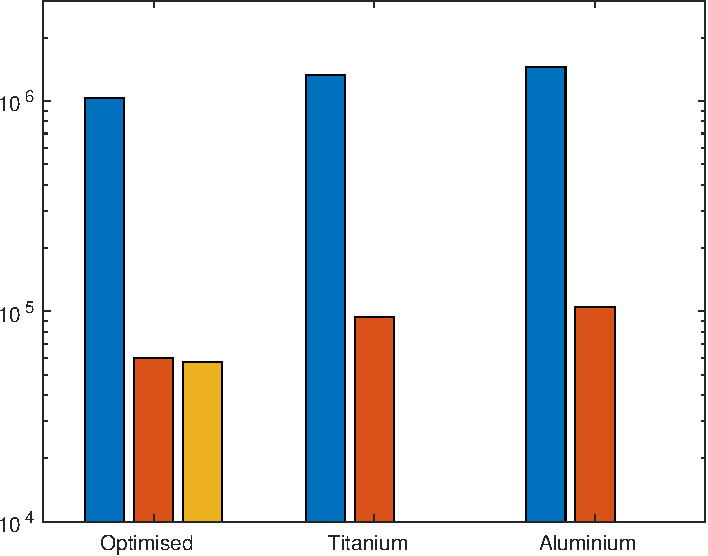
\includegraphics[width=\textwidth]{Media/J_Electron_Shielding}
         \caption{TID for Electrons as Source Particles}
         \label{fig:TIDElectronShielding}
     \end{subfigure}
     \hfill
     \begin{subfigure}[b]{0.49\textwidth}
         \centering
         \includegraphics[width=\textwidth]{Media/J_Proton_Shielding}
         \caption{TID for Proton as Source Particles}
         \label{fig:TIDProtonShielding}
     \end{subfigure}
     \caption{TID of aluminium, titanium, and the optimised radiation structure shown in \autoref{tab:OptimalRadiationProtection} with an weight target of 0.5 \(\text{g/cm}^2\) over 30 days of exposure on Europa}
     \label{fig:AluminiumTitanOptimised}
\end{figure}

\begin{table}[htb]
\centering
\caption{Used components and the respective radiation tolerance and location}
\begin{adjustbox}{max width=\textwidth}
\begin{tabular}[l]{lccccc}

	\toprule
		Components	&	Rated TID	&	Exposed TID	&	Location\\
	\midrule
	
	Electric Motors	&	-	&	< 205 krad	&	locomotion housing\\	
	
	Harness	&	-	&	< 98 krad	&	chassis\\	
	
	Stereo Vision Cams	&	40	&	< 31 krad	&	camera housing\\	
	
	OBC	&	1000	&	< 17 krad	&	E-Bay\\
	
	PCDU	&	20	&	< 17 krad	&	E-Bay\\
	

	\bottomrule

\end{tabular}
\end{adjustbox}
\label{tab:RadiationList}
\end{table}

\begin{figure}[htb]
     \centering
     \begin{subfigure}[b]{0.49\textwidth}
         \centering
         \includegraphics[width=\textwidth]{Media/J_Electron_Compartments}
         \caption{TID for Electrons as Source Particles for different compartments}
         \label{fig:TIDElectronShielding}
     \end{subfigure}
     \hfill
     \begin{subfigure}[b]{0.49\textwidth}
         \centering
         \includegraphics[width=\textwidth]{Media/J_Proton_Compartments}
         \caption{TID for Proton as Source Particles for different compartments}
         \label{fig:TIDProtonShielding}
     \end{subfigure}
     \caption{TID for different compartments}
     \label{fig:CompartmentTID}
\end{figure}

\cleardoublepage
\end{document}























































% Formatierungsoptionen & Dokumenteneinstellungen

%\documentclass[11pt,a4paper,twoside]{report}
%\usepackage[a4paper,left=2.5cm,right=2.5cm, top=2.4cm, bottom=3.2cm]{geometry}
%\usepackage[hang]{caption}
%\usepackage[font={small}]{caption}
%%\usepackage{ucs}
%\usepackage[utf8]{inputenc}
%% Standard Style-Files
%\usepackage{amsmath,amssymb,amsthm}
%\usepackage{a4}
%\usepackage[table,xcdraw]{xcolor}
%\usepackage{graphicx}
%\usepackage{algorithmic,algorithm}
%%\usepackage{subfigure}
%\usepackage{longtable}
%\usepackage[makeroom]{cancel}
%\usepackage[]{placeins}
%\usepackage{adjustbox}
%%Textbox: \begin{textblock*}{29mm}(45mm,80mm)-> h:45mm v:80 von oberen linken Ecke mit 29mm Breite, Höhe durch Inhalt. %Inhalt beliebig(Bilder,Text,..) 
%\usepackage[absolute]{textpos}
%\usepackage{caption}
%\usepackage{lipsum} 
%\usepackage[hidelinks, linktoc = all]{hyperref}
%\usepackage{multirow}
%\usepackage{lscape}
%%\usepackage[official]{eurosym}
%\usepackage[gen]{eurosym}
%\usepackage{subcaption}
%%\usepackage{subfig}
%\usepackage{pdfpages}
%%\usepackage{url}
%\usepackage{listings}
%\usepackage[sorting=none, backend=bibtex, maxbibnames=99, url=true]{biblatex}
%%\usepackage{url}
%%\bibliographystyle{unsrt}
%\usepackage{color} %red, green, blue, yellow, cyan, magenta, black, white
%\definecolor{mygreen}{RGB}{28,172,0} % color values Red, Green, Blue
%\definecolor{mylilas}{RGB}{170,55,241}
%\addbibresource{References}
%
%\interfootnotelinepenalty=10000
%
%\lstset{language=Matlab,%
%	basicstyle=\linespread{0.5}\tiny],
%    %basicstyle=\color{red},
%    breaklines=true,%
%    morekeywords={matlab2tikz},
%    keywordstyle=\color{blue},%
%    morekeywords=[2]{1}, keywordstyle=[2]{\color{black}},
%    identifierstyle=\color{black},%
%    stringstyle=\color{mylilas},
%    commentstyle=\color{mygreen},%
%    showstringspaces=false,%without this there will be a symbol in the places where there is a space
%    numbers=left,%
%    numberstyle={\tiny \color{black}},% size of the numbers
%    numbersep=7pt, % this defines how far the numbers are from the text
%    emph=[1]{for,end,break},emphstyle=[1]\color{red}, %some words to emphasise
%    %emph=[2]{word1,word2}, emphstyle=[2]{style}, 
%    extendedchars=true,
%    literate={µ}{{$\mu$}}1 {η}{{$\eta$}}1 {²}{{$^{2}$}}1 {µm}{{$\mu$m}}1 {µm'}{{$\mu$m '}}1 {μ}{{$\mu$}}1 {π}{{$\pi$}}1 {±}{{$\pm$}}1 ,   
%}
%% ############################################################################
%% Inverse Suche mit xdvi und kile:
%%
%\usepackage{srcltx}
%%
%% 1) xdvi starten mit 
%%    > xdvi -editor 'kile %f --line %l' bericht.dvi
%% 2) Bei einem Klick ins angezeigte dvi-Dokument springt kile automatisch an
%%    die richtige Stelle im latex-file
%
% 
%% Seitenstil
%\pagestyle{headings}
%
%% Abstand zwischen Abs"atzen
%\setlength{\parskip}{1.5ex}
%
%% Einr"uckung der ersten Zeile eines Absatzes unterdr"ucken
%\setlength{\parindent}{0pt}
%
%% Grosszuegigere Wortabstaende
%\sloppy
%
%% Damit Bilder m"oglichst da sind, wo man sie will
%\setcounter{topnumber}{20}
%\setcounter{bottomnumber}{20}
%\setcounter{totalnumber}{20}
%\renewcommand{\topfraction}{.9999}
%\renewcommand{\bottomfraction}{.9999}
%\renewcommand{\textfraction}{0}
%
%
%\newcommand{\chapquoteright}[3]{\begin{quotation} \textit{#1} \end{quotation} \begin{flushright} - #2, \textit{#3}\end{flushright} }
%
%\newcommand{\chapquoteleft}[3]{  \begin{quotation} \textit{#1} \end{quotation} \begin{flushleft}- #2, \textit{#3}\end{flushleft} }
%
%%##########################################################################
%% Bilder:
%% ps/eps-File mit Unterschrift:
%\newcommand{\mypicture}[4]{
%\begin{figure}[hptb]
%\begin{center}
%\includegraphics[scale=1,angle=#4]{#1}
%\caption{#2}\label{#3}
%\end{center}
%\end{figure}
%}%newcommand%
%% Aufruf mit \mypicture{file}{caption}{label}{angle}
%
%% ps/eps-File mit Unterschrift und Angabe der Breite:
%\newcommand{\myscalepicture}[5]{
%\begin{figure}[hptb]
%\begin{center}
%\includegraphics[width=#5,angle=#4]{#1}
%\caption{#2}\label{#3}
%\end{center}
%\end{figure}
%}%newcommand%
%% Aufruf mit \myscalepicture{file}{caption}{label}{angle}{width}
%
%%##########################################################################
%% Tabellen:
%% Gleitende Tabelle:
%\newcommand{\mytable}[3]{
%\begin{table}[hptb]
% \caption{#2}
%  \centerline{#1}
%  \label{#3}
%\end{table}
%}%newcommand%
%% Aufruf mit \mytable{tabelle}{caption}{label}
%
%
%
%%##########################################################################
%% Gleichungs--Referenzen:
%
%% im Text
%\newcommand{\refeqn}[1]{(\ref{#1})}
%% Aufruf mit \refeqn{label}
%
%%##########################################################################
%% Wort-Abkuerzungen:
%
%% \def\abkuerzung/{{text}}
%% Aufruf mit \abkuerzung/
%\def\MKS/{{Mehrk"orpersystem}}
%
%
%%##########################################################################
%% Textmodus
%%##########################################################################
%% Mathematischer Modus 
%
%% Masseinheiten
%\newcommand{\meh}[1]{~\mbox{#1}}
%% Aufruf mit \meh{einheit}
%% Zahlenmengen
%\newcommand{\realR}{{\Bbb{R}}}
%\newcommand{\integerN}{{\Bbb{N}}}
%\newcommand{\complexC}{{\Bbb{C}}}
%
%\newcommand{\fett}[1]{{\mathbf{#1}}}
%% Aufruf mit \realR, \integerN und \complexC
%
%
%%##########################################################################
%% Sonderumgebungen
%\newtheorem{definition}{Definition}[chapter]
%% Aufruf mit \begin{definition}[zusatz]  text  \end{definition}
%\newtheorem{satz}{Satz}[chapter]
%% Aufruf mit \begin{satz}[zusatz]  text  \end{satz}
%
%\theoremstyle{definition}
%\newtheorem{beispiel}{Beispiel}[chapter]
%% Aufruf mit \begin{beispiel}[zusatz]  text  \end{beispiel}
%\newtheorem{algorithmus}{Algorithmus}[chapter]
%% Aufruf mit \begin{algorithmus}[zusatz]  text  \end{algorithmus}
%\floatstyle{ruled}
%\newfloat{algorithm}{thp}{alg} 
%\floatname{algorithm}{Algorithmus}
%
%%###########################################################################
%% Bearbeitung von einzelnen Kapiteln
%
%%\includeonly{02Mission}
%
%%###########################################################################
%
%\begin{document}
%
%%###########################################################################
%
%   Titelseite
%
%###########################################################################

\begin{titlepage}
	
	\begin{textblock*}{117mm}(56mm,30mm)
	%{127mm}(51mm,47mm)
		
		\begin{center}
		
		
			72320 Roversystemtechnik \\
			Summer Semester 2021
			
			\vspace{10mm}
			
			\large \textbf{Phase 0/A-Study of a Rover Mission on the Surface \\ of the Jupiter moon Europa}
			
			\vspace{10mm}
			
			\large \textbf{INSPIRE} \\ 
			\vspace{5mm}
			\large \textbf{IN-situ Sampling and Primal Investigation \\ Rover on Europa}
			
			\vspace{10mm}
			
			\begin{figure}[htb]
    		\centering
     		\includegraphics[width=0.5\textwidth]{Media/Logo}
			\end{figure}
			
			\vspace{10mm}
			
			
			\vspace{10mm}
			
			
			\normalsize 
			Denis Acker \\
			Daniel Bölke \\
			Korbinian Kasper \\
			Christian Korn \\
			Nicolas Probst \\
			Saskia Sütterlin \\
			
			
			\vspace{10mm}
			
			Supervisors: \\
			Moritz Nitz M.Sc. \\
			Patrick Winterhalder M.Sc. 
			
			\vspace{10mm}
			
			University of Stuttgart \\
			Institute of Space Systems \\
			Prof. Dr. Sabine Klinkner \\
			18.07.2021
			
		\end{center}
	
	\end{textblock*}
	
\end{titlepage}



%bericht no IRS-16-035

%  \vspace{10mm} 
%         {\large \hspace{13mm} \\
%         \large \hspace{13mm} \\
%         \large \hspace{13mm} \\
%         \large \hspace{13mm} 72320 Roversystemtechnik\\
%         \centering 
%         \hspace{13mm} Summer Semester 2021\\   }
%  \vspace{10mm}
%
%         {\Large
%          \bf
%          \hspace{20mm} Phase 0/A-Study of a Rover Mission \\} 
%         {\Large
%          \bf
%          \hspace{20mm} on the surface of the Jupiter moon:\\
%          } 
%         {\Large
%          \bf
%          \hspace{20mm} Europa: INSPIRE\\
%          }
% 
%
%  \vspace{30mm}
%         {\large \hspace{20mm}Saskia Sütterlin}\\       
%         {\large \hspace{20mm}Denis Acker}\\
%         {\large \hspace{20mm}Krobinian Kasper}\\
%         {\large \hspace{20mm}Daniel Bölke}\\
%         {\large \hspace{20mm}Nicolas Probst}\\    
%         {\large \hspace{20mm}Christian Korn}\\
%  \vspace{20mm}
%  \makebox[40mm]{\large \hspace{16mm} Supervisor: }\makebox[65mm][l]
%                                   {\large\ Moritz Nitz M.Sc.}
%  \makebox[40mm]{}\makebox[65mm][l]{\large\ Patrick Winterhalder M.Sc.}\\
%
%  \vspace{20mm}
%         {\large \hspace{20mm} University of Stuttgart} \\
%         {\large \hspace{20mm} Institute of Space Systems }\\
%         {\large \hspace{20mm} Prof.\ Dr.\ Sabine Klinkner}\\
%  \vspace{10mm}       
%         {\large \hspace{20mm} 18.07.2021}
%         
%         
%\end{center}
%\end{titlepage}
%
%\clearpage
%\thispagestyle{empty}
%\cleardoublepage
% hier zitat
%*\newpage

%%\textit{\chapquoteright{''Sometimes it was hard to believe that all this had been carried up into space and assembled here five hundred miles above the Earth. I didn't know, until Tim mentioned it casually, that most of the material in the Station had actually come from the Moon. The Moon's low gravity made it much more economical to ship equipment from there instead of from the Earth - despite the fact that Earth was so much closer.''}{Arthur C. Clarke}{Roy Malcolm in Islands in the Sky -- 1952}
%%\begin{figure*}[htb]
%{\centering
%\captionsetup{width=0.8\textwidth}
%\includegraphics[width=0.8\textwidth]{Pictures/LumadiCoverComposite}
%\caption{Lunar massdriver composite image. Footage from Apollo 8 and Apollo 11. Rendering of lunar massdriver 3D models.}
%}
%\end{figure*}
%\FloatBarrier

%\vfill
%\chapquoteright{''Denken Sie groß!''}{Deichkind}{2015}}




%% Inhalt auf der rechten Seite beginnen
%
%
%\strut
%\clearpage
%\thispagestyle{empty}
%\cleardoublepage
%  
%\evensidemargin=2pt
%\oddsidemargin=2pt
%
%
%
%% Zeilenabstand strecken
%\renewcommand{\baselinestretch}{1}\normalsize
%\pagenumbering{roman}
%
%\chapter*{Symbols}

\addcontentsline{toc}{chapter}{Symbols}

\markboth{}{SYMBOLS}

\renewcommand{\arraystretch}{1.2}

\begin{longtable}[l]{lll}

	\textbf{Symbol}	&	\textbf{Definition}	\hspace{8cm}	&	\textbf{Unit}	\\ \\
	
% Latin Symbols

\(a\)					&	Constant for the Geometry of a Porous Media	& nm							\\
\(A\)					&	Wheel Ground Contact Area					& m								\\
\(b\)					&	Wheel Width 								& m								\\
\(c\)					&	Coefficient of Soil Cohesion				& Pa							\\
$C_\text{Batt,req}$		&	Total Required Battery Capacity				& Wh							\\
$C_\text{Batt,req}$		&	Battery Nominal Capacity					& Wh							\\
$C_\text{cell}$			&	Cell Voltage								& V								\\
\(C_\text{rr}\)		&	Rolling Resistance Coefficient					& -								\\	
\(d\)					&	Wheel Diameter								& m								\\
$DoD$					&	Depth of Discharge							& $\%$							\\
\(DP\)					&	Drawbar Pull								& N								\\
\(H\)					&	Soil Thrust									& N								\\
\(h_\text{Ice}\)		&	Ice Crust Surface Thickness on Europa		&	m							\\
\(k_\text{c}\)			&	Sinkage Modulus								& \(\frac{\text{kN}}{\text{m}^{n+2}}\) \\
\(k_\phi\)				&	Soil Friction Angle Sinkage Modulus			& \(\frac{\text{kN}}{\text{m}^{n+3}}\) \\
\(l\)					&	Ground Contact Length						& m								\\
\(T_\text{Surface}\)	&	Surface Temperature on Europa				&	K							\\
$M$						&	Number of Cells in Parallel					& -								\\
$m_\text{RTG}$			&	RTG Mass									& kg							\\
\(n\)					&	Soil Deformation Exponent					& -								\\
$N$						&	Number of Cells in Series					& -								\\
$P_\text{el}$			&	RTG Electrical Power						& $W_\text{el}$					\\
$P_\text{el,req}$		&	Required Electrical Power					& $W_\text{el}$					\\
$P_\text{mode}$			&	Demanded Electrical Power per Mode			& $W_\text{el}$					\\
\(R_\text{b}\)			&	Bulldozing Resistance						& N								\\
\(R_\text{c}\)			&	Compaction Resistance						& N								\\
\(R_\text{g}\)			&	Gravitational Resistance					& N								\\
\(R_\text{r}\)			&	Rolling Resistance							& N								\\
$t_\text{e}$			&	Mode Duration								& s								\\
\(W_\text{wheel}\)		&	Normal Force per Wheel						& N								\\
\(z\)					&	Sinkage										& m								\\


%Greek Symbols


$\alpha_\text{BOL}$		&	BOL Specific Power							& $\frac{W_{el}}{kg}$			\\
\(\epsilon\)			&	Emissivity 									&	-							\\
$\eta_\text{LiIon}$		&	Efficiency of LiIon Cells					& -								\\
\(\phi\)				&	Friciton Angle								& \(^\circ\)					\\
\(\rho_\text{Ice}\)		&	Inner Encoder Ring Diameter  				&	\(\frac{\text{kg}}{m^3}\)	\\
\(\theta\)				&	Slope Angle									& \(^\circ\)					\\






\end{longtable}

\chapter*{Abbreviations}
\addcontentsline{toc}{chapter}{Abbreviations}

\markboth{}{ABBREVIATIONS}

\begin{longtable}[l]{ll}


BOL     & Begin of Life \\
BOM     & Begin of Mission \\
COMM    & Communications \\
C\&DH	& Command \& Data Handling \\
CPU		& Core Processing Unit \\
DoD     & Depth of Discharge \\
EOM     & End of Mission \\
EPS     & Electrical Power System \\
FEC		& Forward Error Correction \\
HGA		& High Gain Antenna\\
LGA		& Low Gain Antenna\\		
2D		& Two Dimensional \\
3D		& Three Dimensional \\
PCDU    & Power Control and Distribution Unit \\
PCU     & Power Control Unit \\
PDU     & Power Distribution and Control Unit \\
IMU     & Inertial Measurement Unit \\
IRS     & Institute of space Systems at the University of Stuttgart \\
INSPIRE & IN-situ Sampling and Primal Investigation Rover on Europa \\
ESA		& European Space Agency	\\
MMP		& Mean Maximum Pressure \\
NASA    &   National Aeronautics and Space Administration \\
SPENVIS	&	SPace ENVironment Information System	\\
HPC     & High Priority Commands \\
RTG     & Radioisotope Thermoelectric Generator \\
eMMRTG  & Enhanced Multi Mission Radioisotope Thermoelectric Generator \\
eSMMRTG & Enhanced and Scaled Multi Mission Radioisotope Thermoelectric Generator (3kg) \\
TID		& Total Ionizing Dose \\
OBC		& On-Board Computer \\
S/C     \\
SBC		& Single Board Computer \\



\end{longtable}

\cleardoublepage






%\addcontentsline{toc}{chapter}{Symbols}
%
%\markboth{}{SYMBOLS}
%
%\renewcommand{\arraystretch}{1.2}
%
%\begin{longtable}[l]{lll}
%  $a$                      & nm                                        & Constant for the Geometry of a Porous Media   \\
%$h_\text{Ice}$           & $\text{km}$,$\text{m}$                      & Ice Crust Surface Thickness on Europa         \\
%$T_\text{Surface}$       & $K$                                         & Surface Temperature on Europa                 \\
%$\epsilon$               & -                                           & Emissivity                                    \\
%$\rho_\text{Ice}$       & $\frac{\text{kg}}{m^3}$                      & Inner Encoder Ring Diameter                   \\
%   
%
%\label{tab:my-table}\\
%\end{longtable}
%
%
%
%
%\chapter*{Abbreviations}
%\addcontentsline{toc}{chapter}{Abbreviations}
%
%\markboth{}{ABBREVIATIONS}
%
%\begin{table}[htb]
%\begin{tabular}[l]{ll}
%PCDU    & Power Control and Distribution Unit \\
%BOL     & Begin of Life \\
%BOM     & Begin of Mission \\
%EOM     & End of Mission \\
%2D		& Two Dimensional \\
%3D		& Three Dimensional \\
%PCU     & Power Control Unit \\
%PDU     & Power Distribution and Control Unit \\
%EPS     & Electrical Power System \\
%IMU     & Inertial Measurement Unit \\
%IRS     & Institute of space Systems at the University of Stuttgart \\
%ESA		&	European Space Agency	\\
%NASA    &   National Aeronautics and Space Administration \\
%SPENVIS	&	SPace ENVironment Information System	\\
%RTG     & Radioisotope Thermoelectric Generator \\
%eMMRTG  & Enhanced Multi Mission Radioisotope Thermoelectric Generator \\
%eSMMRTG & Enhanced and Scaled Multi Mission Radioisotope Thermoelectric Generator (3kg) \\
%TID		& Total Ionizing Dose \\
%
%\end{tabular}
%\end{table}

\cleardoublepage
%%###########################################################################
%
%   Inhaltsverzeichnis
%
%   (wird automatisch erstellt; dieser File ist nicht zu ändern)
%
%###########################################################################


\fancyhead{}
\fancyhead[LE]{\it{CONTENTS}}% LE -> Left part on Even pages
\fancyhead[RO]{\it{CONTENTS}}% RO -> Right part on Odd pages
\tableofcontents
\cleardoublepage

	%default design
	\fancyhead[LE,RO]{\textsl{\rightmark}}
	\fancyhead[LO,RE]{\textsl{\leftmark}}
	\fancyfoot[C]{\thepage}

\fancyhead[ER]{}
\fancyhead[OL]{}
	
\listoffigures
\addcontentsline{toc}{chapter}{\listfigurename}
\clearpage

\listoftables
\addcontentsline{toc}{chapter}{\listtablename}
\cleardoublepage



%\tableofcontents
%\listoffigures
%\listoftables

%
%
%\pagenumbering{arabic}
%%###########################################################################
%
%   Einleitung
%
%###########################################################################
%
\chapter{The Mission}
\label{chap:mission}

During the observation  of Jupiter, the Galileo spacecraft performed flybys of the Jupiter moons, \cite{Mission_01}.
The scientist gathered data from Europa, which supported the evidence of a thick icy surface.
The possibility of liquid water underneath lead astrobiologists to the assumption that extraterrestrial life could exist on Europa, \cite{Mission_02}.
That is why Europa is - beside Mars - an interesting object of research.\\

Therefore, the ESA will launch the \textit{JUICE} orbiter in 2022 to investigate Europa in more detail, \cite{Mission_03}. 
But also the NASA is developing  \textit{Europa Clipper} to get detailed information.
Additionally, they plan a lander for Europer to bring scientific instruments onto the surface, \cite{Mission_04} \cite{Mission_05}.
%There is a side mission planed DLR will perform the side mission \textsc{Technologies for Rapid Ice Penetration and Subglacial Lake Exploration}, with project coordinator Dr. Waldmann, which will take samples of the water by melting through the ice with an special testing probe.\\

Under the leadership of  Prof. Dr.-Ing. Klinkner, the Institute of Aero Space Systems started within a seminar a feasibility study about a rover system to explore Europa surface, which shall  be part of the \textit{TRIPLE} mission.
This challenge was given to five student teams in order to develop concepts, construct preliminary designs, perform analysis and make evaluations to  meet the mission objectives and fit the mandatory requirements cite. \\


This report contains the results of the Phase A study of the rover system \textsc{IN-situ Sampling and Primal Investigation Rover on Europa}  (INSPIRE).
%\chapter{Operation}
\label{chap:Operation}
.....
asdfsdfsadf

%\chapter{Subsystems}
\label{chap:subsystems}
.....



\section{Rover}
\label{sec:rover}
...
\section{Structure and Mechanics}
\label{sec:mechanics}
...
\section{Communications and Command and Data-Handling}
\label{sec:comm}
...
\section{Payload}
\label{sec:payload}
...
\section{Thermal Control}
\label{sec:thermalcontrol}
...
\section{Electrical Power System}
\label{sec:EPS}
The EPS (Electrical Power System) is the subsystem responsible for the electrical power supply of INSPIRE. It consists of four funadmental parts, which are the energy source, the PCDU unit (Power Control and Distribution)and the Energy Storage as well as the rover subsystems as the consumers.

\subsection{EPS Budget and Overview}

\begin{figure}[htb]
{\centering
\includegraphics[width=0.5\textwidth]{Media/epsflowchart}
\caption{Functional Flow Chart Diagram for the EPS Subsystem.}
\label{fig:epsflowchart}
}
\end{figure}

\subsection{Energy Source}
For the energy generation of INSPIRE many possible sources were taken into consideration for a trade-off. The outcome of this trade-off is shown in \autoref{fig:epssourcetradeoff} for the most promising energy sources. As a conclusion of this trad-off the decision was made to utilize a Radioisotope Thermoelectric Generator (RTG) as the main energy source for INSPIRE. \\

As the research couldn't find an RTG with a mass suitable for INSPIRE, the solution was to scale down a bigger RTG as an approximation. As a baseline of the scaling the eMMRTG (Enhanced Multi Mission Radioisotope Thermoelectric Generator) was utilized, which is currently under development at NASA and is especially designed for deep space missions like Europa. For the scaling a goal RTG mass of $m_\text{RTG}=3 \ \text{kg}$ was defined and the eMMRTG was scaled down using the given data.
In \autoref{tab:esmmrtg} the scaling results for the eSMMRTG (Enhanced and Scaled Multi Mission Radioisotope Thermoelectric Generator) are listed. The eSMMRTG has a mass of $m_\text{RTG}=3 \ \text{kg}$ and a BOL specific power of $\alpha_\text{BOL}= 4.0 \ \frac{W_{el}}{kg}$ and provides an electrical power of $P_{el} = 12.08 \ W_{el}$ during the mission duration.



\begin{figure}[htb]
{\centering
\includegraphics[width=0.7\textwidth]{Media/epssourcetradeoff}
\caption{Trade-Off Conclusion for the EPS Energy Source.}
\label{fig:epssourcetradeoff}
}
\end{figure}

\begin{table}[H]
\centering
\begin{tabular}{|c|c|}
\hline
\multicolumn{2}{|c|}{Scaled eSMMRTG Parameter}                \\ \hline
\textbf{System Mass} $m_\text{RTG}$ [$kg$]                             & \textbf{3.5}     \\ \hline
BOL Specific Power $\alpha_\text{BOL}$ $\frac{W_{el}}{kg}$  & $4.0$     \\ \hline
BOL Power $P_{el,\text{BOL}}$ $\ W_{el}$                    & $14$       \\ \hline
Isotrop                                                     & Pu-238   \\ \hline
Isotrop Half-Life [$a$]                                       & $87.7$     \\ \hline
Flight time and Storage (incl. Margins) [$a$]                 & $7$        \\ \hline
Power Loss Degradation until BOM $\ W_{el}$                 & $0.56$     \\ \hline
BOM Power $P_{el,\text{BOM}}$ $\ W_{el}$                    & $13.44$    \\ \hline
Europa Day Duration [$h$]                                     & $85$       \\ \hline
Mission Duration [$d$]                                        & $106.25$   \\ \hline
End of Mission Power $P_{el,\text{EOM}}$ [$\ W_{el}$]         & $13.42$   \\ \hline
\textbf{Final Power for Study} $P_{el}$ [$\ W_{el}$] (incl. $10\%$ scaling Margin) & \textbf{12.08}    \\ \hline

\end{tabular}
\caption{Parameters for the scaled eSMMRTG based on the eMMRTG.}
\label{tab:esmmrtg}
\end{table}

Furthermore INSPIRE will also be equipped with some radiation hardend solar arrays as already explained in \autoref{subsec:radhard}. Since these solar cells are primarily used for technology testing, the mission must also be able to operate completely without this generated energy. For this reason, and because the expected energy generated by the solar cells is minimal, only the energy generated by the RTG is considered for the Phase 0 Study. However, it should be noted that these solar cells will also generate a certain amount of energy, which will benefit the EPS.


\subsection{Energy Storage} 
For the energy storage of INSPIRE many possible battery types were taken into consideration for a trade-off. As a conclusion of this trad-off the decision was made to utilize LiIon batteries as the secondary batteries of INSPIRE. This decision is primarly based on LiIon batteries high energy density, temperature range, robust performance and long operating and cycle life in extreme environemnts. \\
As the RTG only generates a small constant power the main energy source during the mission will be the accumulated energy of the batteries. The rover will charge the batteries at night, so the next exploration day can start with full capacity. Furthermore the batteries have to be charged during day time to maintain operations.\\

For the sizing of the batteries, the rover motion was chosen as the design driver, since this is the highest energy consuming state of the rover and additionally mission critical for INSPIRE. The rover motion consists of an interaction of the Locomotion and Perception mode as already mentioned in \autoref{chap:Operation}. Therefore it was defined that INSPIRE shall be able to drive $ 50 \ m $ (including alternating Locomotion and Perception Mode) with a fully charged Battery. The required Battery Capacity $C_\text{Batt,req}$ can be caculated using \autoref{eq:batreq}. The results are listed in \autoref{tab:batsize}.


\begin{equation}
C_\text{Batt} = \frac{P_\text{el,req} \cdot t_e }{DoD \cdot \eta_\text{LiIon}}
\label{eq:batreq}
\end{equation}

\begin{table}[htb]
\centering
\resizebox{\textwidth}{!}{%
\begin{tabular}{|l|c|c|}
\hline
\textbf{Power Consumption Mode:}                        & \textbf{Locomotion} & \textbf{Perception} \\ \hline
Required Electrical Power $P_\text{el,req}$ [$W_{el}$]         & 283.43              & 14.01               \\ \hline
Duration of the mode$ t_e$ [$s$]                          & 500              & 15000            \\ \hline
$DOD$ for Dimensioning [-]                              & 0.90                & 0.90                \\ \hline
Efficiency of LiIon Cells $\eta_\text{LiIon}$ [-]       & 0.95                & 0.95                \\ \hline
Required Battery Capacity per mode $C_\text{mode}$ [$Wh$] & 46.04               & 68.27               \\ \hline
\textbf{Total Required Battery Capacity} $C_\text{Batt,req}$ [$Wh$]    & \multicolumn{2}{c|}{\textbf{114.32}}               \\ \hline
\end{tabular}%
}
\caption{Power consumption mode used as design case for the battery sizing.}
\label{tab:batsize}
\end{table}

Using these values a suitable battery cell and battery design configuration were conducted. Using these parameters the battery capacity $C_\text{Batt}$ can be calcuated:

\begin{equation}
C_\text{Batt} = C_\text{cell} \cdot V_\text{cell} \cdot N \cdot M .
\label{eq:batuse}
\end{equation}

According to the ECSS reliability restrictions 1 battery string must be substracted for dimensionsing. Furthermore a $30 \%$ margin on the energy content was applied. This leads to a final battery configuration with a capacity of $C_\text{Batt}=138,88 \ Wh$ and a mass of $m = 1980 \ g$. The final battery values are listed in \autoref{eq:batuse}.


% Please add the following required packages to your document preamble:
% \usepackage{graphicx}
\begin{table}[htb]
\centering
\resizebox{\textwidth}{!}{%
\begin{tabular}{|c|c|}
\hline
\multicolumn{2}{|c|}{\textbf{SAFT 176065 xlr}}                                                                \\ \hline
\multicolumn{2}{|c|}{\textbf{Configuration:}}                                                                 \\ \hline
Battery Configuration                                                           & $4s3p$                        \\ \hline
Cells in Sereis $s$ N [-]                                                       & $4$                           \\ \hline
Cells in Parallel $p$ M [-]                                                     & $3$                           \\ \hline
\multicolumn{2}{|c|}{\textbf{Cell Parameters:}}                                                               \\ \hline
Typical Cell Capacity   [$Ah$]                                                    & $6.8$                         \\ \hline
Nominal Cell Voltage [$V$]                                                        & $3.65$                        \\ \hline
Nominal Cell Capacity [$Wh$]                                                      & $24.8$                        \\ \hline
Typical Cell Mass [$kg$]                                                          & $0.15$                        \\ \hline
Energy Density [$Wh/kg$]                                                     & $165.33$                      \\ \hline
\multicolumn{2}{|c|}{\textbf{Actual Battery Configuration Parameters:}}                                       \\ \hline
Battery Voltage $V_\text{Batt}$ [V]                                             & $14.6$                        \\ \hline
Battery Nominal Capacity $E_\text{Batt}$ [$Wh$]                                   & $297.6$                       \\ \hline
Battery Mass [$kg$]                                                               & $1.8$                         \\ \hline
\textbf{Battery Mass} (incl. $10\%$ Margin) [$kg$]                                         & \textbf{1.98}                        \\ \hline
\multicolumn{2}{|c|}{\textbf{Configruation according to ECSS reliability restrictions and margins included:}} \\ \hline
Battery Configuration                                                           & $4s2p$                        \\ \hline
Cells in Sereis $s$ N [-]                                                       & $4$                           \\ \hline
Cells in Parallel $p$ M [-]                                                     & $2$                           \\ \hline
Battery Voltage $V_\text{Batt}$ [$V$]                                             & $14.6 $                       \\ \hline
Battery Nominal Capacity $E_\text{Batt}$ [$Wh$]                                   & $198.4$                       \\ \hline
$30\%$ Margin on Energy Content                                                 & $0.3$                         \\ \hline
\textbf{Battery Nominal Capacity} $E_\text{Batt}$ incl. Margin [$Wh$]                      & \textbf{138.88}                      \\ \hline
Useable Energy Density [$Wh/kg$]                                              & $70.14$                       \\ \hline
\end{tabular}%
}
\caption{INSPIRE battery parameters.}
\label{tab:battery}
\end{table}


\subsection{EPS Power Control and Distribution}
In order to ensure the full functionality of the EPS, the last main component to be selected is a suitable PCDU. As described in \autoref{fig:epsflowchart}, the PCDU forms the heart of the EPS and is also an important interface to the OBC and COMM. Furthermore the PCDU shall be able to monitor and control the rover system if necessary through watchdogs, HPC (High Priority Commands) and direct connections to the OBC and COMM.\\
The PCDU has the challenging task not only to process the RTG as the main energy source, but also to process solar cells as secondary energy sources. Therefore, a PCDU was sought which has the required size, dimensions and range of functions. The research resulted in the Nova PCDU from Bradford DSI. In addition, margins were added to the PCDU to ensure feasibility.

\clearpage

\section{Radiation}
\label{sec:Radiation}

Compared to the radiation environment near Earth the radiation environment near Jupiter is multiple times stronger. It has the highest radiation levels of any planet in our solar systems \cite{Platzhalter}. In order to survive these harsh environmental conditions, special emphasis must be placed on the radiation protection. In \autoref{fig:trappedprotonelectronfluxes}, the average trapped proton and electron fluxes on Europa's orbit around Jupiter are shown in comparison to the outer Van Allen radiation belt around Earth. However, in contrast to the Van Allen radiation belt, the duration within the radiation environment on Europa cannot be minimised and the rover has to be designed to withstand the entire mission duration of 30 days. \\ \\
In oder to design and evaluate different radiation protection approaches, different calculations have to be performed. For this purpose the ESA SPace ENVironment Information System (SPENVIS) is used \cite{Platzhalter}. All calculations and figures in \autoref{sec:Radiation} are performed with SPENVIS unless otherwise stated.

\subsection{Radiation Protection}

Various options are available to protect the rover against the radiation. A common approach is the use of aluminium or titanium as these materials can also act as structural elements. However, due to the mass constraints of 30 kg other materials or material compositions are taken in consideration which are more mass effective. In \autoref{tab:OptimalRadiationProtection}, an optimised shield structure is presented for different weight thresholds designed for the radiation environment around Jupiter.

\begin{wraptable}{r}{8cm}
\centering
\caption{Optimal shield structure for an Jupiter mission. \cite{Platzhalter}}
\begin{adjustbox}{max width=\textwidth}
\begin{tabular}[l]{cccccc}

	\toprule
	
	Areal Density	&	\(0.5\)	&	\(1\) &  \(2\) & \(3\)	\\
	/ \(\text{g/cm}^2\)	&	&	&  & \\
	
	\midrule
	
	
	Layer No. 1	&	Pb &  Pb & W	& Ta	\\
	/ mm	&	0.415 &  0.829 & 0.984	& 1.563	\\
	
	
	Layer No. 2	&	Fe	&  Mg &	Mg & Al \\
	/ mm	&	\(0.033\)	&  \(0.158\) &	\(0.540\) & \(0.399\) \\
	
	
	Layer No. 3 &	-	&  -	& - & Mg \\
	/ mm &	-	&  -	& - & \(0.150\) \\
	

	\bottomrule

\end{tabular}
\end{adjustbox}
\label{tab:OptimalRadiationProtection}
\end{wraptable}

The difference between an aluminium or titanium shielding and an optimised structure listed in \autoref{tab:OptimalRadiationProtection} for the total ionizing dose (TID) is shown in \autoref{fig:AluminiumTitanOptimised}. \\ \\
Due to the mass savings of the optimised structure it will be used where the radiation protection of the aluminium structure is not sufficient. In order to reduce the mass further, a radiation vault is utilised that highly sensible components do not have to be shielded separately.

\subsection{Components}

%TODO Auswahl 0.5 g/cm^2

Every component on the rover has a different radiation tolerance and therefore have to be placed at different compartments within the rover. The radiation tolerances are listed in \autoref{tab:RadiationList}.

\subsection{Improvements}

\subsection{Conclusion}

\clearpage

\section{Locomotion}
\label{sec:locomotion}



\section{Control and Autonomy}
\label{sec:ControlandAutonomy}

\cleardoublepage
%\chapter{Lander System}
\label{chap:lander}
....

\section{Storage Configuration}
\label{sec:storage}
....

\section{Depolyment Strategy}
\label{sec:deployment}
....
%\chapter{Trade-Offs}
\label{chap:tradeoff}
.....
%\chapter{Risk and Technology Assessment}
\label{chap:risks}
.....

 
\section{Risk Assessment}
.....
\subsection{Risk Assessment Subsection}
....

\section{Technology Assessment}
....
\subsection{Acceleration segment}
...
%
%% Quellenverzeichnis über Citavi Anbindung
%
%\include{08Bibilography}
%
%% Wenn benötigt
%%###########################################################################
%
% Anhang
%
%###########################################################################
%\begin{appendix}
%\label{chap:Appendix}
%\chapter{Appendix A}
%\setcounter{chapter}{1}
%\addcontentsline{toc}{chapter}{Appendix}
%###########################################################################
% Anhang A
%###########################################################################
%\label{A}
%....


%\chapter{Appendix B}
%###########################################################################
% Anhang B
%###########################################################################
%\label{B}

%\pagebreak
%###########################################################################
%\end{appendix}

\renewcommand\thesection{\Alph{section}}
\renewcommand\thefigure{\thesection\arabic{figure}}
\renewcommand{\thetable}{\thesection\arabic{table}}
\setcounter{figure}{0}
\setcounter{table}{0}
\setcounter{section}{0}

\chapter*{Appendix}
\addcontentsline{toc}{chapter}{Appendix}

\label{chap:Appendix}

%-------------------------------------------------
\section{Electrical Power System} \label{sec:AppendixEPS}
%-------------------------------------------------
\begin{table}[htb]
\centering
\begin{tabular}{|c|c|}
\hline
\multicolumn{2}{|c|}{\textbf{SAFT 176065 xlr}}                                                                \\ \hline
\multicolumn{2}{|c|}{\textbf{Configuration:}}                                                                 \\ \hline
Battery Configuration                                                           & $4s3p$                        \\ \hline
Cells in Sereis $s$ N [-]                                                       & $4$                           \\ \hline
Cells in Parallel $p$ M [-]                                                     & $3$                           \\ \hline
\multicolumn{2}{|c|}{\textbf{Cell Parameters:}}                                                               \\ \hline
Typical Cell Capacity   [$Ah$]                                                    & $6.8$                         \\ \hline
Nominal Cell Voltage [$V$]                                                        & $3.65$                        \\ \hline
Nominal Cell Capacity [$Wh$]                                                      & $24.8$                        \\ \hline
Typical Cell Mass [$kg$]                                                          & $0.15$                        \\ \hline
Energy Density [$Wh/kg$]                                                     & $165.33$                      \\ \hline
\multicolumn{2}{|c|}{\textbf{Actual Battery Configuration Parameters:}}                                       \\ \hline
Battery Voltage $V_\text{Batt}$ [V]                                             & $14.6$                        \\ \hline
Battery Nominal Capacity $E_\text{Batt}$ [$Wh$]                                   & $297.6$                       \\ \hline
Battery Mass  [$kg$]                                                               & $1.8$                         \\ \hline
\textbf{Battery Mass} $m_\text{Batt}$ (incl. $10\%$ Margin) [$kg$]                                         & \textbf{1.98}                        \\ \hline
\multicolumn{2}{|c|}{\textbf{Configruation according to ECSS reliability restrictions and margins included:}} \\ \hline
Battery Configuration                                                           & $4s2p$                        \\ \hline
Cells in Sereis $s$ N [-]                                                       & $4$                           \\ \hline
Cells in Parallel $p$ M [-]                                                     & $2$                           \\ \hline
Battery Voltage $V_\text{Batt}$ [$V$]                                             & $14.6 $                       \\ \hline
Battery Nominal Capacity $E_\text{Batt}$ [$Wh$]                                   & $198.4$                       \\ \hline
$30\%$ Margin on Energy Content                                                 & $0.3$                         \\ \hline
\textbf{Battery Nominal Capacity} $E_\text{Batt}$ incl. Margin [$Wh$]                      & \textbf{138.88}                      \\ \hline
Useable Energy Density [$Wh/kg$]                                              & $70.14$                       \\ \hline
\end{tabular}
\caption{INSPIRE battery parameters.}
\label{tab:battery}
\end{table}

\begin{figure}[htb]
{\centering
\includegraphics[width=1.0\textwidth]{Media/powerbudgetdummy}
\caption{POWER BUDGET DUMMY!}
\label{tab:powerbudgetcomplete}
}
\end{figure}


%-------------------------------------------------
\section{Thermal Controls System} \label{sec:AppendixThermal}
%-------------------------------------------------
\subsection{Heat energy eqilibrium}

\underline{RTG:}
\[ \dot{Q}_{} = 0  \]\\[2em]

% \dot{Q}_{}
\underline{Electric Bay:}
\[ \dot{Q}_{B,intern}+ CON1 \cdot (T_{RTG}-T_{Bay})+ CON3 \cdot (T_{Chassis}-T_{Bay})  -\epsilon_{alloy}\cdot \sigma_b \cdot S_{Bay}\cdot T_{Bay}^4=0 \]
with: 
\[\dot{Q}_{B,intern} = \dot{Q}_{C\&DH} + \dot{Q}_{Tranceiver} +\dot{Q}_{Receiver} +\dot{Q}_{PCDU} \] \\[2em]

\underline{Drill \& Analyser:}
\[ \dot{Q}_{} = 0  \]\\[2em]

\underline{Camera:}
\[ \dot{Q}_{} = 0  \]\\[2em]

\underline{Radiator:}
\[ \dot{Q}_{} = 0  \]\\[2em]

\underline{Chassis:}
\[ \dot{Q}_{} = 0  \]\\[2em]

\underline{Steer Enine:}
\[ \dot{Q}_{} = 0  \]\\[2em]

\underline{Distribution Node 1:}
\[ \dot{Q}_{} = 0  \]\\[2em]

\underline{Drive Engine:}
\[ \dot{Q}_{} = 0  \]\\[2em]

\underline{Distribution Node 1:}
\[ \dot{Q}_{} = 0  \]\\[2em]


\subsection{Heat conductance}


\subsection{Values}
\begin{table}[htb]
	\centering
	\begin{tabular}{lcc}
		\hline
		 & \multicolumn{2}{l}{Temperature limits in [$^\circ C$]} \\ 
		Component	&	min. & max. \\\hline
		Command \& Data Handling & & \\
		Transmitter & -10 & 50 \\
		Receiver & -30 & 70 \\
		PCDU & -40 & 60 \\
		Battery & -35 & 60 \\
		Camera & -40 & 70 \\
		Objektive  & -40 & 71 \\
		Steering Engine & -30 & 100 \\
		Steering Gear & -30 & 85 \\
		Drive Engine & -40 & 100 \\
		Drive Gear & -40 & 100 \\ \hline
	\end{tabular}
	\caption{Temperatur limits of the rover components.}
	\label{tab:tsc_limits}
\end{table}

\begin{table}[htb]
	\centering
	\begin{tabular}{lccccc}
		\hline
		& \multicolumn{2}{l}{Emisivity [-]} & \multicolumn{2}{l}{Absorptivity [-]}& Source  \\ 
		Surface finishing	&	min. & max. 	&	min. & max.  & \\\hline
		Sand blasted alloy & & & & & \\
		White paint & & & & & \\
	\end{tabular}
	\caption{Minimum and maximum of surface emisivity and absorptivity values.}
	\label{tab:tsc_surface}
\end{table}

\clearpage

\section{Radiation}
\label{sec:AppendixRadiation}

All calculations and figures in \autoref{sec:AppendixRadiation} are performed with SPENVIS unless otherwise stated.

%TODO welche Tools verwendet und welchen Orbit zum simulieren
%TODO letzte Schicht Si
%TODO slap statt squere ausgewählt wegen Eis
%TODO wieviel mm von welchem Material

\begin{figure}[htb]
     \centering
     \begin{subfigure}[b]{0.49\textwidth}
         \centering
         \includegraphics[width=\textwidth]{Media/E_Electron_Flux}
         \caption{Average spectra of trapped electrons around Earth}
         \label{fig:trappedelectronsEarth}
     \end{subfigure}
     \hfill
     \begin{subfigure}[b]{0.49\textwidth}
         \centering
         \includegraphics[width=\textwidth]{Media/E_Proton_Flux}
         \caption{Average spectra of trapped protons around Earth}
         \label{fig:trappedprotonsEarth}
     \end{subfigure}
     \hfill
     \begin{subfigure}[b]{0.49\textwidth}
         \centering
         \includegraphics[width=\textwidth]{Media/J_Electron_Flux}
         \caption{Average spectra of trapped electrons around Jupiter}
         \label{fig:trappedelectronsJupiter}
     \end{subfigure}
     \hfill
     \begin{subfigure}[b]{0.49\textwidth}
         \centering
         \includegraphics[width=\textwidth]{Media/J_Proton_Flux}
         \caption{Average spectra of trapped protons around Jupiter}
         \label{fig:trappedprotonsJupiter}
     \end{subfigure}
     \caption{Average trapped proton and electron fluxes on an orbit around earth at 25,000 km, through the outer Van Allen radiation belt, and on Europa's orbit around Jupiter.}
     \label{fig:trappedprotonelectronfluxes}
\end{figure}

\begin{figure}[htb]
     \centering
     \begin{subfigure}[b]{0.49\textwidth}
         \centering
         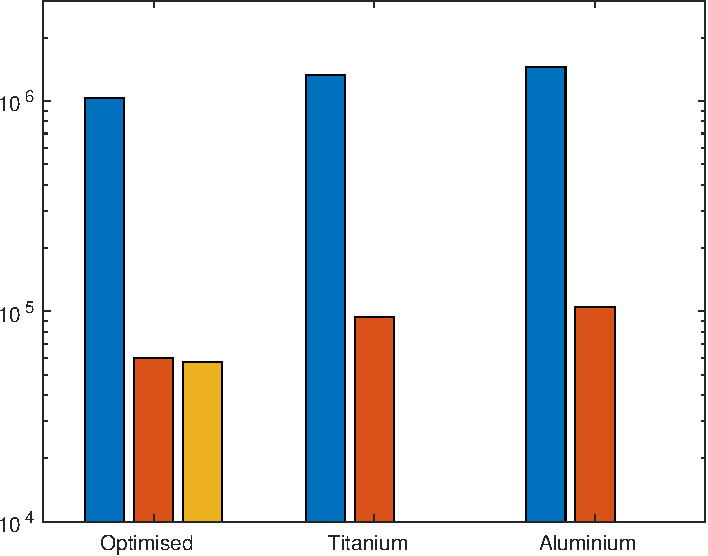
\includegraphics[width=\textwidth]{Media/J_Electron_Shielding}
         \caption{TID for Electrons as Source Particles}
         \label{fig:TIDElectronShielding}
     \end{subfigure}
     \hfill
     \begin{subfigure}[b]{0.49\textwidth}
         \centering
         \includegraphics[width=\textwidth]{Media/J_Proton_Shielding}
         \caption{TID for Proton as Source Particles}
         \label{fig:TIDProtonShielding}
     \end{subfigure}
     \caption{TID of aluminium, titanium, and the optimised radiation structure shown in \autoref{tab:OptimalRadiationProtection} with an weight target of 0.5 \(\text{g/cm}^2\) over 30 days of exposure on Europa}
     \label{fig:AluminiumTitanOptimised}
\end{figure}

\begin{table}[htb]
\centering
\caption{Used components and the respective radiation tolerance and location}
\begin{adjustbox}{max width=\textwidth}
\begin{tabular}[l]{lccccc}

	\toprule
		Components	&	Rated TID	&	Exposed TID	&	Location\\
	\midrule
	
	Electric Motors	&	-	&	< 205 krad	&	locomotion housing\\	
	
	Harness	&	-	&	< 98 krad	&	chassis\\	
	
	Stereo Vision Cams	&	40	&	< 31 krad	&	camera housing\\	
	
	OBC	&	1000	&	< 17 krad	&	E-Bay\\
	
	PCDU	&	20	&	< 17 krad	&	E-Bay\\
	

	\bottomrule

\end{tabular}
\end{adjustbox}
\label{tab:RadiationList}
\end{table}

\begin{figure}[htb]
     \centering
     \begin{subfigure}[b]{0.49\textwidth}
         \centering
         \includegraphics[width=\textwidth]{Media/J_Electron_Compartments}
         \caption{TID for Electrons as Source Particles for different compartments}
         \label{fig:TIDElectronShielding}
     \end{subfigure}
     \hfill
     \begin{subfigure}[b]{0.49\textwidth}
         \centering
         \includegraphics[width=\textwidth]{Media/J_Proton_Compartments}
         \caption{TID for Proton as Source Particles for different compartments}
         \label{fig:TIDProtonShielding}
     \end{subfigure}
     \caption{TID for different compartments}
     \label{fig:CompartmentTID}
\end{figure}

\cleardoublepage
%\end{document}

%##########################################################################
